% ===================================================================
% Chapter 6: Designing the RDT Control System: The Command Conveyor
% ===================================================================

\chapter{Designing the RDT Control System: The Command Conveyor}
\label{chap:rdt_design}

\begin{navigationbox}{In this chapter, you will learn:}
    \begin{itemize}
        \item How the seven fundamental principles of our architecture are applied to the concrete design of the RDT controller.
        \item How to trace the \term{Command Conveyor}: the end-to-end journey of a single user command through all architectural layers of our system.
        \item The conceptual role of each key RDT component (\hcode{Adapter}, \hcode{Planner}, \hcode{MotionManager}, etc.) at each stage of the command lifecycle.
        \item How data is transformed and enriched as it flows "down" from the abstract GUI to the concrete HAL.
        \item How feedback flows "up" from the physical sensors back to the user interface, closing the control loop.
        \item The typical latencies at each stage and how they contribute to the overall system performance and responsiveness.
    \end{itemize}
\end{navigationbox}

In the previous chapter, we studied the fundamental laws that govern all industrial controllers. Now it is time to put these laws into practice. In this chapter, we will design the architecture of our own system—RDT. We will not be diving into the code just yet. Our goal is to create a high-level "map" of the system, define its key components, their responsibilities, and the rules of their interaction. We will use our primary tool of system analysis: we will trace the complete lifecycle of a single command, from a click in the user interface to the rotation of a motor. We call this journey the \textbf{Command Conveyor}.

\section{The Fundamental Principles of Our Architecture}
\label{sec:rdt_principles}

Before we draw schematics or write code, a good architect formulates a set of laws that their system will live by. These laws are not dogma, but conscious choices based on the system's requirements and an analysis of possible trade-offs. The principles we have embedded into the foundation of RDT are not unique; rather, they are the quintessence of time-proven engineering experience, adapted to create a control system that is understandable, implementable, and extensible.

Our architecture stands on seven fundamental pillars:

\begin{enumerate}
    \item \textbf{Separation of Concerns:} Every component does one job and does it well.
    \item \textbf{Determinism First:} Time is the most critical resource; the RT-domain is sacrosanct.
    \item \textbf{Layered Abstraction:} From the general to the specific, hiding complexity at each level.
    \item \textbf{Look-ahead Buffering:} A safety margin for ensuring smooth motion.
    \item \textbf{Asynchronicity for Non-Critical Tasks:} Do not interfere with the main task.
    \item \textbf{Single Source of Truth (SSOT):} Everyone knows everything they need to know, from one verifiable source.
    \item \textbf{Contract-Based Design:} Define clear interfaces and boundaries for all interactions.
\end{enumerate}

These principles do not exist in a vacuum. They are interconnected and form a single architectural fabric, which is depicted in Figure ~\ref{fig:rdt_blueprint}. This diagram is the most important map in this book. We will refer to it again and again as we break down each of its elements in detail.


\begin{figure}[h!] 
    \centering
    \begin{infobox}{The RDT Architecture Blueprint} % Тип блока Infobox для описания структуры
        \textbf{A conceptual diagram of the RDT system architecture.} % Пояснительный текст

        \begin{lstlisting}[
            language=Text,              
            basicstyle=\ttfamily\footnotesize, 
            columns=fixed,              
            frame=none,                 
            numbers=none,               
            showstringspaces=false,   
            breaklines=false,           
            breakatwhitespace=false,    
            xleftmargin=0pt,           
            infobox
            xrightmargin=0pt,           
            infobox
            aboveskip=0.5cm,            
            belowskip=0.5cm             
        ]
----------------- Integration Layer (NRT) -----------------------
            [GUI Panels (Panel_Teach, ...)]    
              || (Qt Signals/Slots) ||
             [Adapter_RobotController]

------ Coordination & Computation Layer (NRT / Soft-RT) --------
               [RobotController (Orchestrator)]
             /                 ||               \
[TrajectoryPlanner] <-> [StateData (SDO)] <-> [KdlKinematicSolver]
              ||  (Motion Profile)  ||
                         V
              [TrajectoryInterpolator]

------------- Execution Layer (RT) ----------------------------
[TrajectoryQueue (Command Buffer)]   <-- Planner writes here
              | |
               V
     [MotionManager (RT-Cycle)]
              | | (IMotionInterface contract)
               V
     [HAL (Fake/UDPMotionInterface)]
              | |
               V
[TrajectoryQueue (Feedback Buffer)]  --> RobotController reads here
        \end{lstlisting}
    \end{infobox}
    \caption{The complete architectural map of the RDT system, showing key components and their primary data flow paths. This blueprint will be our guide for the rest of the book.}
    \label{fig:rdt_blueprint}
\end{figure}


Let us now explore the essence of each of these seven principles in the context of our RDT architecture.

% --- Continuation of 6.1 ---

\subsection{The Pillars of RDT's Architecture}
\label{subsec:rdt_pillars}

\paragraph{1. Separation of Concerns (SoC)}
This is the most fundamental principle of software engineering, which states that a system should be decomposed into parts with minimal overlap in functionality. In RDT, this is not an abstract guideline but a strict rule enforced at every level. Each component has a single, well-defined responsibility.
\begin{itemize}
    \item The \textbf{TrajectoryPlanner} thinks about geometry and time. It knows how to build a smooth path between two points and how to respect velocity limits. It knows nothing about Qt signals, motor drivers, or network protocols. Its world is pure mathematics.
    \item The \textbf{Adapter\_RobotController} is a pure translator. It knows how to convert a Qt signal from a button click into a well-formed C++ command for the \hcode{RobotController}. It does not perform any kinematics or path planning. Its only job is to bridge the worlds of the GUI framework and the C++ core.
    \item The \textbf{MotionManager} is a metronome. Its sole responsibility is to maintain the real-time cycle and shuttle data between the command buffer and the hardware abstraction layer. It does not know what a "linear" or "joint" move is; for it, all commands are just a set of joint coordinates that must be sent out on time.
\end{itemize}
This strict separation is what allows us to develop, test, and replace any component in the system with minimal cascading changes to other parts.

\paragraph{2. Determinism First}
As we established in the previous chapter, the real-time (RT) domain operates under a different set of physical laws than the non-real-time (NRT) domain. In our architecture, we rigorously enforce this separation.
\begin{itemize}
    \item \textbf{NRT-Domain (The Thinkers):} This includes everything from the GUI down to the \textbf{TrajectoryPlanner}. This is where all the "heavy" and unpredictable operations happen: solving inverse kinematics, parsing user programs, rendering 3D graphics, and updating the UI.
    \item \textbf{RT-Domain (The Doer):} This consists solely of the \hcode{MotionManager}. It executes simple, predictable code within a hard real-time loop. It \textit{never} waits for the NRT-domain.
\end{itemize}

\begin{principlebox}{Determinism: A Non-Negotiable for Smooth and Safe Motion}
    The cost of this determinism is a deliberate limitation of functionality within the RT-domain. This is not a flaw; it is a critical, non-negotiable design decision.
\end{principlebox}

\paragraph{3. Layered Abstraction}
The system is structured as a hierarchy of layers, where each higher-level layer utilizes the functionality of a lower-level layer through a well-defined interface, without knowing its internal implementation. This is analogous to the OSI model in networking: the application layer doesn't know how the physical layer encodes bits into electrical signals; it simply requests the "send data" service.
\begin{itemize}
    \item The \textbf{RobotController} orchestrates the \hcode{TrajectoryPlanner} but does not know \textit{how} it plans.
    \item The \textbf{MotionManager} consumes setpoints from a queue but does not know who produced them.
    \item Most importantly, the \textbf{MotionManager} commands the robot by talking to an abstract \hcode{IMotionInterface}, not to a specific hardware driver.
\end{itemize}
This abstraction is the key to creating a \textbf{Digital Twin}. We can easily switch the system's behavior from a simulation to a real robot simply by providing the \hcode{MotionManager} with a different implementation of the \hcode{IMotionInterface} contract—for instance, swapping \hcode{FakeMotionInterface} for \hcode{UDPMotionInterface}. Not a single line of code in the \hcode{MotionManager} or any layer above it needs to change.

% --- Continuation of 6.1 ---

\paragraph{4. Look-ahead Buffering}
To sever the direct temporal dependency between the fast, deterministic RT-cycle and the slower, unpredictable NRT-planner, we use a look-ahead buffer. In our architecture, this is implemented by the \hcode{TrajectoryQueue} class. It acts as a shock absorber, or a spring, between the two domains.
\begin{itemize}
    \item The \textbf{Producer (NRT-Planner)} works at its own pace. It calculates the trajectory not just for the next step, but for a significant time into the future (e.g., 100-500 ms) and places the resulting stream of setpoints into the buffer. Its job is to ensure the buffer is always sufficiently filled.
    \item The \textbf{Consumer (RT-MotionManager)} operates in its strict, periodic cycle (e.g., every 2 ms). In each cycle, it simply retrieves one pre-calculated setpoint from the front of the buffer and sends it for execution. It always has a supply of work ready.
\end{itemize}

\begin{tipbox}{The Buffer Size Trade-off.}
    The size of the look-ahead buffer is a critical architectural compromise.
    \begin{description}
        \item[A small buffer (e.g., 20-50 ms):] Provides high \textit{responsiveness}. The robot reacts quickly to a `Stop` command because there are few "old" commands in the pipeline that need to be executed first. However, it offers low \textit{resilience} to NRT-domain delays; even a small "freeze" of the planner can drain the buffer and cause motion to stutter.
        \item[A large buffer (e.g., 500-1000 ms):] Provides high \textit{resilience}. The system can survive significant NRT-domain delays without interrupting smooth motion. However, it results in low \textit{responsiveness} ("sluggishness"). When an operator presses `Stop`, the robot will first execute up to a full second of already planned movements, which can be unacceptable or even dangerous.
    \end{description}
    In industrial controllers, the buffer size is often a configurable parameter, tuned by the integration engineer for the specific task.
\end{tipbox}

\paragraph{5. Asynchronicity for Non-Critical Tasks}
Any task that does not have hard real-time guarantees and could potentially block or delay execution must run asynchronously to the core control loop. This principle protects the determinism of the RT-domain.
\begin{itemize}
    \item \textbf{GUI Updates:} The Qt event loop runs in its own main thread. It periodically polls \hcode{StateData} for changes, but its rendering delays or event processing never affect the \hcode{MotionManager}'s RT thread.
    \item \textbf{Logging to Disk:} A truly robust logging system would not write to a file directly from a core component. It would push log messages into another lock-free queue, and a dedicated, low-priority logger thread would be responsible for slowly consuming messages from that queue and writing them to a file, never blocking the main application logic.
\end{itemize}
This ensures that a slow disk, a network timeout, or a complex UI repaint will never cause a catastrophic failure in the robot's motion control.

% --- Continuation of 6.1 ---

\paragraph{6. Single Source of Truth (SSOT)}
Instead of allowing components to communicate with each other directly, creating a "spaghetti" architecture of dependencies, all communication about the system's state within the NRT-domain happens through a centralized, thread-safe data store. In our architecture, this is the \textbf{StateData} object, an implementation of the \textit{Blackboard} architectural pattern.
\begin{itemize}
    \item \textbf{Writers:} Components write the results of their work to the `StateData` object. The \hcode{Adapter} writes the user's intent (e.g., selected tool). The \hcode{RobotController} writes the results of feedback processing (e.g., current TCP pose).
    \item \textbf{Readers:} Components read the data they need from the `StateData` object. The \hcode{TrajectoryPlanner} reads the active tool to perform its calculations. The \hcode{GUI} reads the current TCP pose to update the 3D view.
\end{itemize}
This radically decouples the components. The \hcode{TrajectoryPlanner} does not need to know about the existence of the \hcode{GUI}, and vice-versa. They only need to know about the `StateData` object and the data contract it provides. This guarantees that at any moment, all parts of the system are operating on a consistent snapshot of the system's state.

\begin{dangerbox}{The Peril of Direct Communication.}
    What happens if we violate this principle? Imagine the \hcode{GUI} needs to know the current joint angles. It could make a direct call to a method in the \hcode{KdlKinematicSolver}. This single "convenient" shortcut creates a toxic dependency. The GUI is now tied to the Kinematics module. It becomes impossible to test the GUI without a kinematics solver. A change in the solver's interface could break the GUI. This is how unmaintainable monoliths are born.
\end{dangerbox}

\paragraph{7. Contract-Based Design}
Interaction between components and layers is defined not by concrete classes, but by abstract interfaces—\textbf{contracts}. A component depends on the \textit{behavior} guaranteed by an interface, not the specific \textit{implementation} that provides it.
\begin{itemize}
    \item The \hcode{MotionManager} depends on the \hcode{IMotionInterface} contract, not on the \hcode{Fake MotionInterface} or \hcode{UDPMotionInterface} classes.
    \item The \hcode{TrajectoryPlanner} depends on the \hcode{KinematicSolver} contract, not on the \hcode{Kdl KinematicSolver} class.
\end{itemize}
This is the principle that enables maximum flexibility, extensibility, and, crucially, testability. We can provide a "mock" or "fake" implementation of any interface to test a component in complete isolation. We can add support for a brand new robot in the future simply by writing a new class that implements the \hcode{IMotionInterface} contract, without changing a single line of code in the core system.

\vspace{1cm} % Add some space before the concluding paragraph
These seven principles are the DNA of the RDT architecture. They are not arbitrary rules but engineering solutions to the fundamental problems of building complex, real-time systems: managing complexity, ensuring predictability, and planning for future evolution. In the following sections, we will see how this DNA expresses itself at each stage of the Command Conveyor.

%%%\lipsum[4] % Placeholder text

% ===================================================================
% Section 6.2: The Robot's Heartbeat: The Industrial Control Loop
% ===================================================================

\section{The Robot's Heartbeat: The Industrial Control Loop}
\label{sec:control_loop}

At the core of any autonomous agent's behavior, from a simple insect to a sophisticated industrial robot, lies a continuous feedback loop. The agent constantly senses the world, plans its actions based on these perceptions and its goals, acts upon that plan, and then senses the results of its actions to adjust its subsequent behavior. This fundamental process is known as the \textbf{Sense-Plan-Act} cycle. It is the very "heartbeat" of any intelligent system. Let's break down its classical stages:

\begin{enumerate}
    \item \textbf{Sensing:} The robot continuously "senses" its own state and its environment. Of paramount importance is the data from encoders on each joint, which provide a high-precision measurement of the robot's current joint configuration. In addition, other sensors can be used: force/torque sensors, machine vision systems, external position sensors, and so on.
    
    \item \textbf{Planning:} Based on the data about its current state and a given target (or an entire trajectory), the controller performs calculations to determine exactly how the robot should move. This is where algorithms for kinematics, trajectory planning, interpolation, and constraint checking come into play. This is the "thinking" part of the cycle.
    
    \item \textbf{Actuation:} The calculated target motion parameters (e.g., desired positions or torques for each joint) are converted into control signals. These signals are sent to the executive devices—the servo drives—which power the robot's joints, striving to achieve the commanded parameters.
\end{enumerate}

The cycle then closes: the result of the action is immediately read by the sensors, this new state information is fed back into the system's input, and the entire process repeats at a very high frequency—from hundreds to thousands of times per second.

\subsection{Distributing the Cycle in an Industrial Architecture}
\label{subsec:distributing_the_cycle}

In a simple educational robot, all three stages (Sense, Plan, Act) might be executed sequentially within a single loop. However, as we established in the previous chapter, this is impossible in a high-performance industrial controller. The "Planning" stage is a computationally intensive and unpredictable task in terms of time. Forcing it into the same rigid, real-time cycle as "Sensing" and "Acting" would be a recipe for disaster, destroying the very determinism we seek to achieve.

Therefore, in mature architectures, and specifically in our RDT system, this cycle is \textbf{distributed} between the RT and NRT domains.

\begin{tipbox}{Analogy: The Human Reflex Arc}
    Consider what happens when you touch a hot stove.
    \begin{itemize}
        \item \textbf{Sense \& Act (Spinal Cord, RT-Domain):} Receptors in your skin (sensors) send a signal to your spinal cord. The spinal cord, without waiting for instructions from the brain, instantly sends a reflexive command to your muscles (actuators) to pull your hand away. This is an ultra-fast, deterministic, life-saving RT-cycle.
        \item \textbf{Plan (Brain, NRT-Domain):} Only \textit{after} your hand is already safe does the pain signal reach your brain. And only then does the complex processing begin: "What was that? A stove. Why was it hot? I turned it on. What should I do next? Blow on my fingers and don't touch it again." This is a complex, asynchronous planning process.
    \end{itemize}
    Our controller operates on the exact same principle: fast, simple reflexes are separated from slow but intelligent planning. This is not just an elegant analogy; it's a fundamental architectural pattern for building robust real-time systems.
\end{tipbox}

As shown in Figure~\ref{fig:distributed_cycle}, the stages of the cycle in our RDT system are distributed as follows:

\begin{itemize}
    \item \textbf{PLAN: Entirely in the NRT-Domain.} All the "heavy" intellectual work is performed here, without strict time constraints. 
    \begin{itemize}
        \item \textit{Components Responsible:} \hcode{TrajectoryPlanner} and \hcode{KdlKinematicSolver}.
        \item \textit{Primary Task:} To take a high-level command (e.g., "move to P1 linearly") and decompose it into a long sequence of low-level setpoints (target joint positions for each RT-cycle tick).
        \item \textit{The Result:} Filling the look-ahead buffer (\hcode{TrajectoryQueue}) with ready-to-execute commands.
    \end{itemize}

    \item \textbf{SENSE \& ACT: Entirely in the RT-Domain.} Only fast, deterministic execution happens here.
    \begin{itemize}
        \item \textit{Components Responsible:} \hcode{MotionManager} and the underlying Hardware Abstraction Layer (\hcode{IMotionInterface}).
        \item \textit{The ACT Task:} In each cycle, take one setpoint from the buffer and send it to the servo drives.
        \item \textit{The SENSE Task:} In each cycle, read the actual state from the servo drives (joint positions, torques) and send it back up to the NRT-domain for logging and display.
    \end{itemize}
\end{itemize}

\begin{figure}[htbp!] % Изменено на [htbp!] для большей гибкости размещения фигуры
    \centering
    \begin{infobox}{The Distributed Sense-Plan-Act Cycle in RDT} % Основной Infobox для диаграммы
        \textbf{Projection of the Sense-Plan-Act Cycle onto the RT/NRT Architecture}
        
        \textbf{NRT-Domain (The Brain)}
        \begin{infobox}{PLAN: Trajectory Planning, IK Solving, Logic} % Вложенный Infobox
            \textit{Components: TrajectoryPlanner, RobotController}
        \end{infobox}
        
        % ASCII-арт для стрелок
        \begin{lstlisting}[language=Text, basicstyle=\ttfamily\scriptsize, columns=fixed, frame=none, numbers=none, showstringspaces=false, breaklines=false, breakatwhitespace=false, aboveskip=0.0cm, belowskip=0.0cm]
     | | (Setpoint Stream via Look-ahead Buffer) | |
     V A (Feedback Stream via Feedback Buffer) A V
        \end{lstlisting}
        
        \textbf{RT-Domain (The Spinal Cord)}
        \begin{infobox}{SENSE: Read encoders, currents, etc. <--> ACT: Send commands to drives} % Вложенный Infobox
            \textit{Components: MotionManager, HAL}
        \end{infobox}
        
        % ASCII-арт для стрелок
        \begin{lstlisting}[language=Text, basicstyle=\ttfamily\scriptsize, columns=fixed, frame=none, numbers=none, showstringspaces=false, breaklines=false, breakatwhitespace=false, aboveskip=0.0cm, belowskip=0.0cm]
     | (Physical Interface) |
     V
        \end{lstlisting}
        
        \textbf{Physical World (Robot Hardware)}
    \end{infobox}
    \caption{How the classic Sense-Plan-Act cycle is split between the Non-Real-Time (NRT) and Real-Time (RT) domains in the RDT architecture. The PLAN phase is complex and asynchronous, while the SENSE and ACT phases form a tight, deterministic loop.}
    \label{fig:distributed_cycle}
\end{figure}

\begin{principlebox}{The Key Architectural Insight.}
    This distribution allows us to achieve two seemingly contradictory goals. We get the rich functionality and planning flexibility of the NRT-domain, and at the same time, the iron-clad determinism and smooth motion of the RT-domain. The look-ahead buffer (\hcode{TrajectoryQueue}) is the crucial link—the shock absorber—that makes their coexistence possible. Understanding this distributed nature of the control loop is the key to understanding the entire architecture.
\end{principlebox}

%%%\lipsum[5] % Placeholder text

% --- Continuation of 6.2 ---

\subsection{The "World Model" and Its Keepers}
\label{subsec:world_model}

This distributed model introduces another critical concept: the "world model" or system state. Since the \textbf{PLAN} and \textbf{SENSE/ACT} parts of the cycle are decoupled in time, they operate on slightly different views of the world.

\begin{itemize}
    \item \textbf{The RT-Domain's View:} The \hcode{MotionManager} has the most up-to-date, real-time information about the physical hardware, which it receives directly from the HAL. However, this view is very low-level (raw encoder ticks, motor currents). It has no concept of a "Tool Center Point" or a "linear move."
    \item \textbf{The NRT-Domain's View:} The \hcode{RobotController} and \hcode{TrajectoryPlanner} operate on a richer, more abstract model of the world stored in the \hcode{StateData} object. This model contains not only the latest feedback from the RT-domain but also higher-level information: the active tool, the active user coordinate system, the overall program state, etc. This view is always slightly delayed compared to the RT-domain's view, but it's more comprehensive and meaningful.
\end{itemize}

The continuous flow of data in the feedback loop (\hcode{HAL -> MotionManager -> Feedback Queue -> RobotController -> StateData}) is the mechanism that keeps the NRT-domain's world model synchronized with physical reality. The latency of this feedback loop is a critical system characteristic, as it determines how quickly the "brain" can react to what the "body" is experiencing.

This understanding of the distributed control loop and its interaction with the shared world model provides the necessary context for our next step: a detailed journey along the Command Conveyor, where we will trace a single command through each of these components and layers.

%%\lipsum[6-7] % Placeholder text

% ===================================================================
% Section 6.3: The Command Lifecycle: A Signal's Journey Through Our System
% ===================================================================

\section{The Command Lifecycle: A Signal's Journey Through Our System}
\label{sec:command_lifecycle}

Now we are ready for the main journey of this book. We will follow a single command from its inception as a mouse click on the screen to its final expression as the physical motion of the robot. This path, which we call the \textbf{Command Conveyor}, passes through all the layers of our architecture. Analyzing each stage of this conveyor will allow us to understand not only \textit{what} each component does, but \textit{why} it does it that way and in that specific place.

\subsection{Stage 1: Intent and Input (The GUI and the Adapter)}
\label{subsec:stage1_gui_adapter}

Everything begins with an operator's intent. The operator wants to teach a new point, jog the robot 10 mm along the X-axis, or start a program. They express this intent through interaction with the Graphical User Interface (GUI).

\paragraph{The Role of the GUI Panels: The "Dumb" Data Source}
In our RDT architecture, the components responsible for interacting with the user are classes inherited from \hcode{QWidget}, such as \hcode{Panel\_JogControl} or \hcode{Panel\_Teach}. Their task is extremely simple and strictly limited. They are the system's eyes and ears, but not its brain.

\begin{dangerbox}{The Golden Architectural Rule: The GUI Must Be "Dumb".}
    There must be no business logic whatsoever within the GUI classes. A \hcode{Panel\_JogControl} must not know what "kinematics" or a "trajectory" is. It must not attempt to calculate the new robot pose itself. Its \textbf{sole responsibility} is to report the user's raw, uninterpreted actions. It should say: "The user clicked the '+X' button on the Jog panel, the step value was '10.0', and the selected frame in the dropdown was 'Tool'." All logic for interpreting this event is delegated to the next layer.
\end{dangerbox}

Why is this separation so critical?
\begin{itemize}
    \item \textbf{Testability:} It allows us to test the entire system core without ever launching a graphical interface. We can simulate user actions by calling the public methods of the next layer (the Adapter) directly.
    \item \textbf{Reusability:} The core logic is not tied to a specific GUI framework (like Qt). If tomorrow we decide to create a web interface using a different technology, we would only need to replace the GUI panels and the Adapter, leaving the entire system core untouched.
    \item \textbf{Maintainability:} It prevents the GUI from becoming a monolithic monster that mixes display logic with complex robotics calculations, which is a common fate of many poorly designed systems.
\end{itemize}

In practice, when a user clicks a button, like "Teach" on the \hcode{Panel\_Teach}, the class simply gathers the raw data from the widgets (motion type, tool name, speed) and emits a Qt signal, for instance, \hcode{teachCurrentPoseRequested(motionType, toolName, ...)}. At this point, its job is done.

\paragraph{The Role of the Adapter: The Validator, Translator, and Formalizer}
The Qt signal from the GUI panel is caught by a central component of the integration layer—in our architecture, this is the \textbf{Adapter\_RobotController}. This is where the real work of this stage begins. The Adapter acts as a gateway and a translator between the "Qt world" (signals, QStrings, QVariants) and the "C++ world" (strongly-typed objects, business logic). It performs three crucial tasks:

\begin{enumerate}
    \item \textbf{Receiving Raw Data:} The Adapter's Qt slot receives the raw arguments from the GUI's signal.
    
    \item \textbf{Enriching with Context from the SDO:} The Adapter understands that the raw data from the GUI is insufficient to form a complete command. To know \textit{from where} to move, it needs to know the robot's current state. It turns to the \hcode{StateData} object (our Single Source of Truth) and "pulls" the latest available information, such as the current joint configuration (\hcode{feedback.joint\_actual}) and the current Cartesian pose (\hcode{feedback.cartesian\_actual}).
    
    \item \textbf{Transformation and Validation:} The Adapter's most important function is to transform the raw, untrusted data into a strictly typed, validated, and complete command object.
    \begin{itemize}
        \item A \hcode{QString("Gripper")} is converted into a \hcode{ToolFrame} object, possibly by looking it up in a configuration database of available tools.
        \item Input values are validated. What if the user entered a speed of \hcode{200\%}? The Adapter must either clamp it to \hcode{100\%} or reject the command as invalid. What if the selected tool does not exist? The Adapter must handle this error gracefully.
    \end{itemize}
    
    \item \textbf{Formalizing the Command:} This is the key step. The Adapter gathers all the data—from the GUI's signal and from the \hcode{StateData} object—and packages it into a single, standardized data structure that will be used throughout the rest of the Command Conveyor. In our architecture, this is the \textbf{TrajectoryPoint} object.
\end{enumerate}


% --- Continuation of 6.3.1 ---

\begin{tipbox}{Engineering Insight: The Creation of the \hcode{TrajectoryPoint}}
\small
The \hcode{TrajectoryPoint} object, created and populated by the Adapter, is the \textbf{first formal artifact} of our Command Conveyor. It contains the complete description of the operator's intent, enriched with all the necessary context. A fully populated \hcode{TrajectoryPoint} at this stage holds the answers to several critical questions:
\begin{itemize}
    \item \textbf{What to do?} \hfill \textit{e.g., \hcode{header.motion\_type = LIN, PTP...}}
    \item \textbf{Where to go?} \hfill \textit{e.g., \hcode{command.cartesian\_target} or \hcode{command.joint\_target}}
    \item \textbf{In which coordinate system?} \hfill \textit{e.g., \hcode{header.base\_frame} specifies the user-selected coordinate system}
    \item \textbf{With which tool?} \hfill \textit{e.g., \hcode{header.tool\_frame} specifies the active tool}
    \item \textbf{With what parameters?} \hfill \textit{e.g., \hcode{command.speed\_percent}, etc.}
    \item \textbf{From where?} \hfill \textit{The current robot state, now implicitly part of the context for the next stage}
\end{itemize}
It is crucial to understand that at this stage, all coordinates in the \hcode{TrajectoryPoint} object are still in the "user's world"—that is, relative to the coordinate systems selected in the GUI. The transformation into the robot's base coordinate system will be the job of the next component on the conveyor.
\end{tipbox}

\paragraph{Launching the Conveyor}
Once the \hcode{TrajectoryPoint} object is fully formed and validated, the Adapter performs its final task at this stage: it hands over control to the system's core. It calls a method on the \hcode{RobotController} (our orchestrator), for example, \hcode{executeMotionToTarget(command)}, passing the newly created command object.

This method call is the moment the command leaves the integration layer and travels further down the conveyor to the next stage—the NRT-core for transformation and planning.

\begin{figure}[htbp!] % Изменено на [htbp!] для большей гибкости размещения фигуры
    \centering
    \begin{infobox}{Data Flow in Stage 1: From Raw Input to Formalized Command} % Тип блока Infobox для описания структуры
        % Используем lstlisting для точного сохранения форматирования ASCII-диаграммы.
        % basicstyle=\ttfamily\scriptsize: моноширинный шрифт уменьшенного размера для лучшей вместимости.
        % columns=fixed: критически важно для выравнивания ASCII-арта.
        % breaklines=false: запрещаем автоматические переносы строк внутри диаграммы.
        \begin{lstlisting}[
            language=Text, % Язык текста, чтобы не было подсветки синтаксиса
            basicstyle=\ttfamily\scriptsize,
            columns=fixed,
            frame=none, % Не рисуем рамку вокруг самого листинга
            numbers=none, % Не нумеруем строки
            showstringspaces=false, % Не показываем пробелы символами
            breaklines=false, % Важно: не переносим строки!
            breakatwhitespace=false, % Не разбиваем строки на пробелах
            aboveskip=0.5cm, % Добавляем небольшой отступ сверху для читаемости
            belowskip=0.5cm % Добавляем небольшой отступ снизу
        ]
Conceptual Data Flow Diagram for Stage 1

[GUI Panels] ---- (Qt Signal: "Jog +X", "10.0") ---> [Adapter]
   ^                                                   |
   | (GUI Reads State for Display)                     | (Adapter Reads Context)
   |                                                   V
[StateData (SDO)] <------------------------------------+
   ||                                                  |
 current_fb_pose                                       V
 active_tool                                [Create & Validate TrajectoryPoint]
                                                        |
                                                        V
[RobotController] <--- (C++ Method Call: executeMotionToTarget(tp)) ---
\end{lstlisting}
    \end{infobox}
    \caption{The data flow at Stage 1 of the Command Conveyor. The Adapter acts as a central hub, gathering raw user input from the GUI and contextual state from the SDO to produce a single, well-defined \hcode{TrajectoryPoint} command object, which is then passed to the system core.}
    \label{fig:stage1_data_flow}
\end{figure}


\subsubsection{Summary of Stage 1}
\label{subsubsec:stage1_summary}

At this first stage of the command lifecycle, a key transformation has occurred:
\begin{itemize}
    \item \textbf{From What:} From a disparate, unstructured, and untrusted collection of data entered by a user into a graphical interface.
    \item \textbf{To What:} Into a single, strictly-typed, validated, and context-enriched command object, the \hcode{TrajectoryPoint}.
\end{itemize}

All the complexity of validation, type conversion, and state retrieval has been encapsulated within the Adapter. This leaves the GUI components maximally simple and the system core completely independent of the details of the UI implementation. The command is now ready for the next, most computationally intensive stage—planning.

%%\lipsum[8-9] % Placeholder text

% ===================================================================
% Subsection 6.3.2: Stage 2: Transformation and Planning (The NRT-Core)
% ===================================================================

\subsection{Stage 2: Transformation and Planning (The NRT-Core)}
\label{subsec:stage2_planning}

Our command, neatly packaged into a \hcode{TrajectoryPoint} object, has left the integration layer. It now enters the most computationally intensive and intelligent part of the system: the Non-Real-Time (NRT) core. The primary task of this layer, and specifically of the \textbf{TrajectoryPlanner} component, is to convert the high-level user intent ("go to this point with this tool") into a low-level, detailed motion plan that the RT-core can understand and execute.

This plan is not a single command but a dense sequence of setpoints—target positions for each robot joint for every single tick of the real-time cycle. This complex process can be visualized as an internal "assembly line" or pipeline within the planner, consisting of several distinct steps.

\begin{figure}[h!]
    \centering
    % For this diagram, we need tikz library
    % Make sure you have \usepackage{tikz} in your preamble
    % and the following libraries
    \usetikzlibrary{shapes.geometric, arrows.meta, positioning, fit}

    \begin{tcolorbox}[
        width=\textwidth,
        halign=center,
        title=The TrajectoryPlanner's Internal Processing Pipeline,
        fonttitle=\bfseries
    ]
    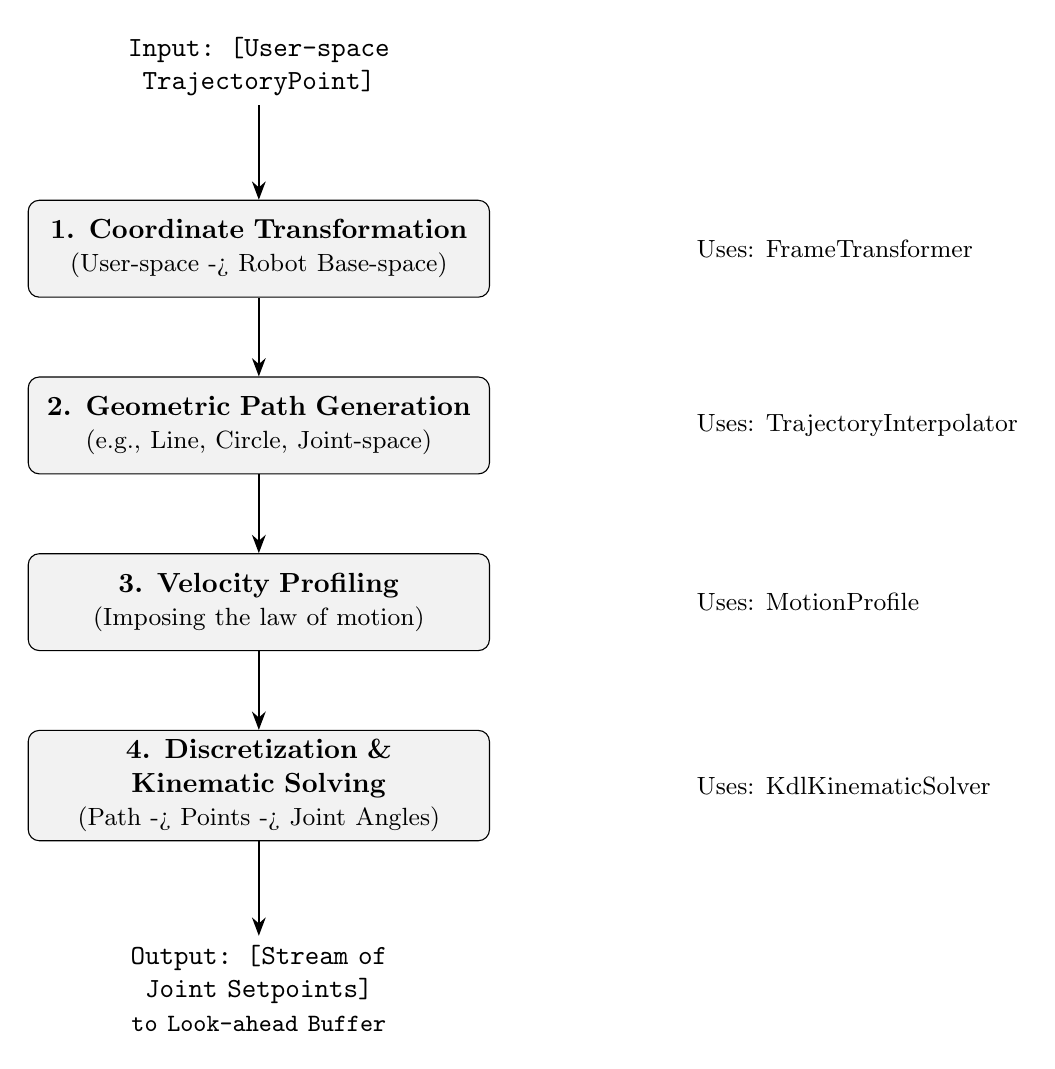
\begin{tikzpicture}[
        node distance=1cm and 2.5cm, % vertical and horizontal
        >=Stealth,
        stage/.style={
            rectangle, 
            draw, 
            fill=gray!10, 
            text width=16em, 
            text centered, 
            rounded corners, 
            minimum height=3.5em
        },
        io/.style={
            text width=16em,
            text centered,
            font=\ttfamily
        },
        uses_note/.style={
            align=left,
            font=\small
        },
        line/.style={draw, -{Stealth}, thick}
    ]
        % Define Nodes for the pipeline
        \node[io] (input) {Input: [User-space TrajectoryPoint]};
        
        \node[stage, below=1.2cm of input] (stage1) {
            \textbf{1. Coordinate Transformation} \\
            \small\hcode{(User-space -> Robot Base-space)}
        };
        
        \node[stage, below=of stage1] (stage2) {
            \textbf{2. Geometric Path Generation} \\
            \small\hcode{(e.g., Line, Circle, Joint-space)}
        };
        
        \node[stage, below=of stage2] (stage3) {
            \textbf{3. Velocity Profiling} \\
            \small\hcode{(Imposing the law of motion)}
        };
        
        \node[stage, below=of stage3] (stage4) {
            \textbf{4. Discretization \& Kinematic Solving} \\
            \small\hcode{(Path -> Points -> Joint Angles)}
        };
        
        \node[io, below=1.2cm of stage4] (output) {Output: [Stream of Joint Setpoints] \\ \small to Look-ahead Buffer};

        % Define "Uses" annotations
        \node[uses_note, right=of stage1] {Uses: \hcode{FrameTransformer}};
        \node[uses_note, right=of stage2] {Uses: \hcode{TrajectoryInterpolator}};
        \node[uses_note, right=of stage3] {Uses: \hcode{MotionProfile}};
        \node[uses_note, right=of stage4] {Uses: \hcode{KdlKinematicSolver}};

        % Draw connecting arrows for the pipeline
        \path[line] (input) -- (stage1);
        \path[line] (stage1) -- (stage2);
        \path[line] (stage2) -- (stage3);
        \path[line] (stage3) -- (stage4);
        \path[line] (stage4) -- (output);
        
    \end{tikzpicture}
    \end{tcolorbox}
    \caption{The internal command processing pipeline within the \hcode{TrajectoryPlanner}. A single high-level command goes through multiple stages of transformation and calculation to produce a stream of low-level, executable setpoints.}
    \label{fig:planner_pipeline}
\end{figure}

Let's examine each step of this internal conveyor in detail.

\paragraph{Step 1: Context and Preparation}
Before any calculations begin, the planner must understand its starting context. It has received the \textit{target} command, but it also needs to know the \textit{current} state of the robot. It queries the \hcode{StateData} object to get the latest feedback pose, which serves as the starting point for the new motion segment. This ensures that every new motion is planned from the robot's actual last known position, providing a seamless transition between movements.

\paragraph{Step 2: Coordinate Transformation — From the User's World to the Robot's World}
The command has arrived as a target pose defined in a user-specified coordinate system (a "User Frame" or "Work Object") and with a specific tool (TCP). The robot's kinematic model, however, only understands one thing: the position and orientation of its \textbf{flange} (the mounting plate at the end of its arm) relative to its own \textbf{base}.

The first critical task is to answer the question: \textit{"To get the specified TCP to the target pose, where must the robot's flange be located in the robot's base coordinate system?"}

This is a purely geometric problem, and it is solved by our \textbf{FrameTransformer} utility. A two-part transformation takes place:
\begin{enumerate}
    \item \textbf{From User Frame to Robot Base:} The target TCP pose is first transformed from the user-selected coordinate system (e.g., the corner of a workpiece) into the robot's "world" or base coordinate system. This is done by multiplying the point by the transformation matrix of the User Frame, which is stored in \hcode{StateData}.
    \item \textbf{From TCP to Flange:} Now that we know where the TCP needs to be in the robot's base frame, we must calculate the corresponding pose for the flange. This is achieved by applying the \textit{inverse} of the tool transformation. If the tool transformation describes how to get from the flange to the TCP (\(T_{flange \to tcp}\)), its inverse describes how to get from the TCP back to the flange (\(T_{tcp \to flange}\)).
\end{enumerate}

\begin{tipbox}{Engineering Insight: Working with the Flange, Not the TCP.}
    A crucial design choice in almost all industrial controllers is that the core motion planning and kinematics operate on the \textbf{flange pose}, not the TCP pose. Why?
    \begin{itemize}
        \item \textbf{Universality:} The robot's kinematic model is a fixed mathematical description that ends at its flange. It knows nothing about the hundreds of different grippers, welders, or sensors that might be attached to it. By transforming the target into a flange pose first, we decouple the "robot math" from the "tool math."
        \item \textbf{Uniformity:} This allows the system to use a single, powerful Forward and Inverse Kinematics solver for all tasks. Information about the tool is only used at the very beginning (to calculate the flange target) and at the very end (to display the resulting TCP position in the GUI). The core remains clean and tool-agnostic.
    \end{itemize}
\end{tipbox}

The result of this stage is two well-defined poses (start and end), both describing the robot's \textbf{flange} in the robot's \textbf{base coordinate system}. All information about user frames and tools is no longer needed for the subsequent calculations. We have successfully translated the problem from the "human's world" to the "robot's world."

% --- Continuation of 6.3.2 ---

\paragraph{Step 3: Geometric Path Generation}
Now that we have a start and an end flange pose in a unified coordinate system, we must define the geometric shape of the path between them. This task is handled by the \textbf{TrajectoryInterpolator}. It looks at the motion type specified in the command's header (\hcode{header.motion\_type}) and constructs the appropriate path.
\begin{itemize}
    \item \textbf{For LIN (Linear) Motion:} The interpolator constructs a straight-line segment in 3D Cartesian space between the start and end flange poses. For the orientation, it creates a path for the smoothest and shortest rotation using Spherical Linear Interpolation (SLERP) on quaternions, as we discussed in Chapter~\ref{chap:language_of_space}.
    \item \textbf{For PTP (Point-to-Point) / JOINT Motion:} In this case, the Cartesian path of the flange is irrelevant. The primary goal is to move the joints from their start to their end configurations. The interpolator will work directly with the joint angles. The path becomes a straight line in the multi-dimensional \textit{joint space}. In the real 3D world, this results in a smooth, curved, but generally unpredictable path of the flange.
    \item \textbf{For CIRC (Circular) Motion:} The interpolator would construct a circular arc that passes through the start, end, and an intermediate "via" point, after all three have been transformed into the robot's base coordinate system.
\end{itemize}

The result of this stage is the "skeleton" of the trajectory—a pure geometric curve (or a set of joint angles) in space, but as of yet, with no concept of time, speed, or acceleration. We know \textit{where} the robot must go, but not \textit{when} or \textit{how fast}.

\paragraph{Step 4: Velocity Profiling — Imposing the Law of Motion}
The next task is to superimpose a law of motion onto this geometric path. An object with mass cannot start or stop instantaneously. It must accelerate and decelerate. This is the job of the \textbf{MotionProfile} component, which is typically part of the \hcode{TrajectoryInterpolator}.

Based on the total path length and the speed and acceleration parameters from the command, it calculates a velocity profile. As discussed in Chapter~\ref{chap:anatomy_of_motion}, this is almost always an \textbf{S-Curve (Jerk-Limited) profile} in modern controllers to ensure smooth motion and minimize mechanical stress. This profile defines exactly what the robot's speed should be at any given moment in time along the trajectory.

\begin{tipbox}{Engineering Insight: Synchronizing Axes in Joint Moves.}
    In a PTP (joint-space) move, each joint has to travel its own, different angular distance. Joint 1 might need to move 10 degrees, while Joint 2 needs to move 50 degrees. How does the system ensure they both start and stop at the same time?
    
    The velocity profile generator finds the "leading axis"—the joint that has to travel the largest distance. It then calculates the velocity profile (e.g., S-curve) for this single axis, ensuring it moves at its maximum permissible speed. Then, it proportionally scales down the speeds of all other axes so that their total travel time matches the travel time of the leading axis. The result: all joints arrive at their destination perfectly synchronized. This is a fundamental technique for coordinated joint motion.
\end{tipbox}

The result of this stage is a complete, time-parameterized trajectory. We can now ask the interpolator: "Give me the target flange pose, velocity, and acceleration at time \(t = 0.125\) seconds," and it will provide an exact answer. The plan is now fully defined in continuous time.

% --- Continuation of 6.3.2 ---

\paragraph{Step 5: Discretization and Kinematic Solving}
The plan is complete, but it's continuous. The RT-core, however, operates in discrete time steps (ticks). The final step of the planning pipeline is to "slice" this continuous trajectory into a sequence of discrete setpoints, one for each tick of the RT-cycle. This is where the planner loops, repeatedly calling the interpolator for the next time step (\(t, t+dt, t+2dt, \dots\)).

With a sampling frequency of 500 Hz (a 2 ms RT-cycle), a 5-second motion will be discretized into 2500 individual points. For each of these points, a final and crucial operation must be performed:

\begin{itemize}
    \item \textbf{For JOINT/PTP Motion:} The task is simple. The interpolator directly provides the target joint angles for each time step. No further kinematic calculations are needed.
    \item \textbf{For LIN/CIRC Motion:} This is the moment of truth. The interpolator provides the target \textit{Cartesian pose} of the flange for each time step. For each of these hundreds or thousands of points, we must now solve the \textbf{Inverse Kinematics (IK) problem} to find the corresponding joint angles that will achieve that specific flange pose. This is the job of the \textbf{KdlKinematicSolver}.
\end{itemize}

\begin{dangerbox}{Performance and Error Handling in IK Solving.}
    This is the most computationally demanding step in the entire planning process. For a 5-second move at 500 Hz, the IK problem must be solved 2500 times! This is why the performance of the IK solver is absolutely critical.
    
    Furthermore, the planner must be prepared for the IK solver to fail. For a given point, a solution might not exist (it's outside the robot's workspace), or it might lie in a singularity. A robust planner must not crash. It must detect this failure, stop the trajectory generation, and report a clear error message (e.g., "Target unreachable at segment time 2.34s"). Sending a path with an unreachable point to the RT-core would be a recipe for undefined behavior.
\end{dangerbox}

After this final step, the transformation is complete. We have successfully converted a single, high-level, user-centric command into a stream of hundreds of low-level, machine-centric, ready-to-execute \hcode{TrajectoryPoint} objects. Each of these objects now contains the target \textbf{joint angles} for a specific RT-cycle tick.

\subsubsection{Summary of Stage 2}
\label{subsubsec:stage2_summary}

At this most complex stage, a fundamental transformation has occurred:
\begin{itemize}
    \item \textbf{From What:} From a single, high-level command object representing a goal in the user's coordinate system.
    \item \textbf{To What:} To a dense stream of hundreds of low-level setpoint objects, each containing the precise joint angles for the robot for a specific, discrete moment in time.
\end{itemize}
All the complexity of coordinate transformations, path geometry, velocity profiling, and inverse kinematics has been handled here, in the NRT-domain, to maximally offload the real-time core. The stream of setpoints is now ready to be sent to the next stage for execution.

%%\lipsum[10] % Placeholder text


% ===================================================================
% Subsection 6.3.3: Stage 3: Preparing for Execution (Buffering) - UPDATED
% ===================================================================

\subsection{Stage 3: Preparing for Execution (Buffering)}
\label{subsec:stage3_buffering_rdt_expanded}

The \hcode{TrajectoryPlanner} has performed its complex task, transforming a single high-level command into a stream of hundreds of low-level, kinematically-solved setpoints. A direct, synchronous handover of this data to the RT-core is architecturally forbidden, as it would tether the predictable RT-domain to the unpredictable NRT-domain.

To create a robust, asynchronous bridge, we introduce this third, crucial logistical stage of our conveyor: \textbf{Buffering}. Here, the stream of "finished parts" from the planner is placed onto a "conveyor belt" before it reaches the real-time assembly line. In our RDT architecture, this role is fulfilled by the \textbf{\hcode{TrajectoryQueue}} class, a specialized lock-free queue.

\begin{navigationbox}{The Role of Buffering: A Quick Recap.}
    As we discussed in detail in Section~\ref{sec:look_ahead_buffer}, the look-ahead buffer is the cornerstone of our distributed architecture. It decouples the NRT and RT domains, absorbs the timing jitter of the planner, and enables advanced features like path blending. We will now focus on the practical implementation of this concept within RDT.
\end{navigationbox}

\paragraph{What Exactly is Placed in the Buffer?}
It is essential to understand the precise data packet that the \hcode{TrajectoryPlanner} enqueues. It's not just an array of joint angles. It is a fully-formed \hcode{TrajectoryPoint} object, meticulously prepared for the RT-core.

\begin{figure}[htbp!]
    \centering
    \begin{tcolorbox}[
        width=\textwidth, 
        sharp corners, 
        title=The Setpoint Data Structure,
        fonttitle=\bfseries
    ]
    
    \begin{center}
    \textbf{Anatomy of a \texttt{TrajectoryPoint} as an RT Setpoint}
    \end{center}
    
    % Листинг 1: Основная структура
    % Настраиваем listings для C++
    % Убедитесь, что \usepackage{listings} и \usepackage{xcolor} есть в преамбуле
    % и определены стили, например:
    % \lstset{language=C++, basicstyle=\ttfamily\small, ...}
    
    \begin{lstlisting}[language=C++, basicstyle=\ttfamily\small]
// The main container for a single point in a trajectory
struct TrajectoryPoint {
    // Contains metadata like sequence index, motion type, etc.
    TrajectoryPointHead Header;
    
    // The actual command data for this setpoint
    RobotCommandFrame   Command;
    
    // Placeholder for feedback data (filled in by RT-core later)
    RobotFeedbackFrame  Feedback; 
};
    \end{lstlisting}
    
    \hrule\vspace{0.2cm} % Горизонтальный разделитель для ясности
    
    % Листинг 2: Вложенная структура с акцентами
    \begin{lstlisting}[language=C++, basicstyle=\ttfamily\small]
// Key data payload inside RobotCommandFrame
struct RobotCommandFrame {
    AxisSet pose_joint; // <-- PRIMARY DATA for RT-Core
    Pose    pose_cart;  // <-- Diagnostic data
};
    \end{lstlisting}
    
    \end{tcolorbox}
    \caption{The structure of the \hcode{TrajectoryPoint} object as it is placed into the \hcode{TrajectoryQueue}. The primary payload for the RT-core is the calculated joint angles (\hcode{pose\_joint}). The Cartesian pose is included for diagnostics and feedback pairing.}
    \label{fig:setpoint_structure_listing}
\end{figure}

As shown in Figure~\ref{fig:setpoint_structure}, while the object is complex, the RT-core will only care about one field: \hcode{command.pose\_joint}. All other information serves diagnostic or feedback purposes, ensuring that we never lose context as data flows through the system.

\paragraph{The Logic of Buffer Management: The Orchestrator's Role}
The \hcode{TrajectoryPlanner} is a "specialist" — it's brilliant at math but doesn't manage its own workload. The logic of \textit{when} to run the planner and \textit{how many} points to generate is managed by a higher-level component, the \textbf{\hcode{RobotController}}. This orchestrator implements the "planning in windows" strategy we introduced earlier.

Its control loop, running in the NRT-domain, can be summarized as follows:
\begin{enumerate}
    \item \textbf{Check Buffer Level:} The \hcode{RobotController} checks the current size of the \hcode{Trajectory Queue}.
    \item \textbf{Check Planner Status:} It also checks if the \hcode{TrajectoryPlanner} has finished processing the current motion segment.
    \item \textbf{Request New Window:} If the buffer has sufficient free space (e.g., is less than 80\% full) AND the current segment is not yet done, it calls \hcode{planner->getNextWindow OfPoints(...)}.
    \item \textbf{Enqueue the Window:} It takes the returned vector of \hcode{TrajectoryPoint} objects and pushes them one by one into the \hcode{TrajectoryQueue}.
    \item \textbf{Wait and Repeat:} It then waits for its next cycle (e.g., 50 ms) before repeating the check.
\end{enumerate}
This creates a simple but effective control system where the \hcode{RobotController} acts as a manager, ensuring the \hcode{TrajectoryPlanner} is always working just enough to keep the \hcode{TrajectoryQueue} supplied, preventing both underrun and overrun conditions.

\begin{tipbox}{Why a Lock-Free Queue is a Must-Have.}
    The choice of a lock-free Single-Producer, Single-Consumer (SPSC) queue for our \hcode{TrajectoryQueue} is a deliberate and critical architectural decision. It is the only way to guarantee that the NRT-planner (the single producer) and the RT-core (the single consumer) can access the buffer without ever blocking each other. This completely eliminates the risk of priority inversion at this critical system boundary, a problem that could bring a mutex-based system to a halt. The detailed implementation of this lock-free queue, with its atomic operations and memory barriers, is a fascinating topic we will dissect in Chapter~\ref{chap:code_dissection}.
\end{tipbox}

\subsubsection{Summary of Stage 3}
\label{subsubsec:stage3_summary_expanded}
At the buffering stage, no new data is created, and no mathematical transformations occur. It is a purely logistical step that finalizes the preparation for real-time execution.
\begin{itemize}
    \item \textbf{The Result:} A stream of fully calculated, low-level setpoints is safely and asynchronously transferred from the NRT-domain into a high-performance, non-blocking queue, ready for consumption by the RT-domain.
    \item \textbf{Key Decisions:}
    \begin{itemize}
        \item The use of a central orchestrator (\hcode{RobotController}) to manage the planning workload in discrete "windows".
        \item The implementation of the buffer as a lock-free SPSC queue to ensure a safe and deterministic bridge between the asynchronous NRT world and the synchronous RT world.
    \end{itemize}
\end{itemize}

The conveyor belt is now fully loaded with precisely manufactured parts. The real-time assembly line has a guaranteed supply of work. We are now ready to enter the metronome-like world of the RT-core.


% ===================================================================
% Subsection 6.3.4: Stage 4: Real-Time Execution (The RT-Core)
% ===================================================================

\subsection{Stage 4: Real-Time Execution (The RT-Core)}
\label{subsec:stage4_rt_core}

We are now at the threshold of the most critical part of our conveyor: the real-time execution core (RT-core). This is where abstract plans and sequences of numbers are transformed into physical action. All the complexity and unpredictability of the NRT-domain have been left behind. The task of the RT-core, which in our project is represented by the \textbf{MotionManager} class, is not to think, but to execute simple, pre-prepared commands with iron-clad precision and predictability.

The operation of the RT-core is an endless, strictly periodic cycle. If the cycle period is set to 2 milliseconds (a frequency of 500 Hz), it \textit{must} complete all its operations and go to sleep until the next tick, exactly 2 ms later. Any deviation from this timing, known as jitter, is a failure of the real-time system.

\paragraph{Anatomy of a Single RT-Tick}
Let's dissect what happens within a single, fleeting cycle of the \hcode{MotionManager}, which lasts only a few milliseconds. The logic is executed in a precise, unvarying sequence.

    \begin{infobox}{Anatomy of a Real-Time Tick}
        \textbf{Timeline of Operations within a Single RT-Cycle}
        \vspace{0.5cm}
        
        \hcode{
        Time: 0.0 ms --- Wake Up (Timer Interrupt) \\
        V \\
        Time: 0.1 ms --- Step 1: Dequeue Command (try\_pop from TrajectoryQueue) \\
        |                +-- Success? Use new command. \\
        |                +-- Failure (Queue Empty)? Use last valid command (Hold Position). \\
        V \\
        Time: 0.2 ms --- Step 2: Validate Setpoint (Basic sanity checks) \\
        V \\
        Time: 0.3 ms --- Step 3: Send Command to HAL (call sendCommand()) --> ACT \\
        V \\
        Time: 0.8 ms --- Step 4: Read Feedback from HAL (call readState()) --> SENSE \\
        V \\
        Time: 0.9 ms --- Step 5: Enqueue Feedback (try\_push to FeedbackQueue) \\
        V \\
        Time: 1.0 ms --- Step 6: Go to Sleep (wait for next timer interrupt) \\
        V \\
        Time: 2.0 ms --- End of Cycle / Next Wake Up \\
        }

    \caption{The sequence of operations inside a single, deterministic RT-cycle. The entire sequence, from waking up to going back to sleep, must complete within the cycle's strict deadline (e.g., 2 ms).}
    \label{fig:rt_tick_anatomy}
    \end{infobox}

Let's break down the logic of these key steps.

\paragraph{Step 1: Waking Up and Dequeuing a Command}
The cycle does not begin with work, but with waiting. The RT-thread is in a sleep state. It is awakened with high precision by the operating system's real-time scheduler at the exact start of the next tick.

\begin{tipbox}{Engineering Insight: High-Resolution Timers and Watchdogs.}
    \begin{itemize}
        \item \textbf{Synchronization Tick:} This precise awakening is not achieved with a standard \hcode{sleep()} function, which is highly non-deterministic. In a real-time OS (RTOS) or a Linux system with the \hcode{PREEMPT\_RT} patch, this is handled by high-resolution timers (e.g., a system call like \hcode{clock\_nanosleep()}) that guarantee minimal jitter.
        \item \textbf{Watchdog Timer:} Concurrently, the system must verify that the previous cycle was not "late". A hardware or software \textbf{watchdog timer} is used for this. Before going to sleep, the RT-core "pets" the watchdog. If the core fails to pet the watchdog on time (because the previous cycle took too long and overran its deadline), the watchdog "bites," triggering a critical system error. This is the primary mechanism for detecting a catastrophic failure or overload of the RT-core.
    \end{itemize}
\end{tipbox}

Immediately upon waking, the \hcode{MotionManager} attempts to retrieve the next command by calling \hcode{try\_pop()} on the \hcode{TrajectoryQueue}. This is a critical moment where one of two things can happen.

% --- Continuation of 6.3.4 ---

\begin{itemize}
    \item \textbf{Success Case (Buffer is not empty):} The \hcode{try\_pop()} operation successfully retrieves a new \hcode{TrajectoryPoint}. This is the normal, expected path of execution. The \hcode{MotionManager} now has a fresh setpoint with new target joint angles. It flags that it has an active command and proceeds.
    
    \item \textbf{Failure Case (Buffer Underrun):} The \hcode{try\_pop()} operation returns false, indicating that the command queue is empty. This is a non-nominal but expected situation. The NRT-planner has, for some reason, failed to keep the buffer supplied. The RT-core \textbf{must not} simply stop or do nothing. This would cause the servo drives to lose power, and the robot arm would slump under gravity. Instead, it enters a safe \textbf{Hold Position} mode.
\end{itemize}

\paragraph{The Hold Position Mechanism: A Safety Net for Motion}
The "Hold Position" mode is a crucial safety feature of the RT-core. When the command buffer runs dry, the \hcode{MotionManager} does not simply give up. It retrieves the \textit{last successfully sent command} from its internal state and prepares to re-send that same command to the HAL.

The effect is that the robot physically freezes in its last commanded position. Its motors remain energized and actively resist any external forces (like gravity), holding the pose. This is infinitely safer than a sudden power-off of the drives. The system will remain in this "hold" state, re-sending the same setpoint in every cycle, until a new command eventually appears in the queue.

\begin{dangerbox}{A Critical Distinction: When to go Idle.}
    The system only transitions to a true \hcode{Idle} state (where the hold logic is no longer active) if the buffer is empty \textbf{and} there was no previously active command. This happens at the very end of a program. In all other cases of buffer underrun during motion, it enters \hcode{Hold Position}. This prevents the robot from being disabled by transient delays in the NRT-domain and is a fundamental aspect of graceful degradation in a control system.
\end{dangerbox}

\paragraph{Step 2-3: Validation and Actuation (Sending the Command)}
After either retrieving a new command or deciding to re-use the last one, the \hcode{MotionManager} performs a few last-minute, extremely fast sanity checks on the setpoint data (e.g., checking if the values are not NaN or infinity).

Then, it performs its primary \textbf{ACT} function: it sends the command to the next layer down the stack, the Hardware Abstraction Layer. It does this by calling the method on its abstract interface:
\hcode{iface->sendCommand(current\_setpoint.command);}

The RT-core does not know, nor does it care, how this method is implemented. Whether it involves writing to shared memory for a simulator, formatting a CAN bus packet, or building an EtherCAT frame is the responsibility of the concrete HAL implementation. The RT-core's only job is to call this method on time.

\paragraph{Step 4-5: Sensing and Feedback (Closing the Local Loop)}
Immediately after sending the command, the RT-core performs its \textbf{SENSE} function. It queries the HAL for the latest actual state of the hardware:
\hcode{RobotStateFrame hal\_fb = iface->readState();}

This call returns the most recent data from the encoders, current sensors, and status flags of the drives.

\begin{tipbox}{Engineering Insight: Command-Feedback Pairing and Latency.}
    It is vital to understand that the feedback received from \hcode{readState()} is not the result of the command that was just sent in the \textit{same} cycle. Due to network and processing latencies in the drives, the feedback always corresponds to a command sent one or more cycles \textit{in the past}.
    
    A sophisticated controller architecture must account for this \textbf{feedback latency}. The \hcode{MotionManager} in our RDT architecture does this by pairing the outgoing command with the incoming feedback. It takes the command it just sent and the feedback it just received and packages them together into a single \hcode{TrajectoryPoint} object. This object, which now contains both the \hcode{Command} and \hcode{Feedback} data for a specific moment in time (or more accurately, for a specific RT-tick), is then pushed into the \hcode{feedback\_queue\_} for the NRT-domain to analyze. This pairing is essential for tasks like calculating the following error or any other analysis that needs to compare what was commanded with what actually happened.
\end{tipbox}

\paragraph{Step 6: Sleeping Until the Next Cycle}
Having completed all its tasks, the RT-thread calculates the time elapsed since it woke up. It subtracts this duration from the total cycle period and then puts itself to sleep for the exact remaining time. This frees up the CPU for other tasks (including the NRT-planner) and ensures that it will wake up precisely at the beginning of the next tick to repeat the cycle all over again.

\subsubsection{Summary of Stage 4}
\label{subsubsec:stage4_summary}

This stage is the system's metronome, where the rhythm of the architecture is established.
\begin{itemize}
    \item \textbf{The Result:} One setpoint from the buffer has been sent for execution, and the corresponding feedback about the robot's physical state has been captured and sent back up the chain for analysis.
    \item \textbf{Key Decisions:}
    \begin{itemize}
        \item The use of high-resolution timers and watchdogs to maintain strict periodicity and detect overruns.
        \item The implementation of a safe "Hold Position" mode to gracefully handle buffer underrun conditions.
        \item The complete isolation from planning logic; the RT-core is a pure, high-fidelity executor, not a thinker.
        \item The use of a lock-free queue to safely receive commands without blocking or risking priority inversion.
    \end{itemize}
\end{itemize}

The command has now been executed. But the command lifecycle is not yet complete. The system must now understand what happened as a result of this action and communicate that information back to the user. This is the journey we will trace in the final stages of the conveyor.

%\lipsum[13-14] % Placeholder text











% ===================================================================
% Subsection 6.3.5: Stage 5: Interfacing with "The Metal" (The HAL)
% ===================================================================

\subsection{Stage 5: Interfacing with "The Metal" (The HAL)}
\label{subsec:stage5_hal}

In the previous stage, we saw the \hcode{MotionManager} (the RT-core) issue commands like \hcode{sendCommand()} and \hcode{readState()} to an abstract object it knows only as \hcode{IMotionInterface}. What is this interface? This is our Hardware Abstraction Layer (HAL). The HAL is one of the most important boundaries in our entire architecture. It is the line that separates the clean, platform-agnostic world of our control logic from the messy, diverse, and complex world of physical hardware.

Why can't the \hcode{MotionManager} just talk directly to the hardware? Why do we need this extra layer of indirection? Imagine a system without a HAL. The \hcode{MotionManager}'s code would be filled with hardware-specific details:
\begin{itemize}
    \item \hcode{write\_to\_ethercat\_pdo(domain, alias, offset, value);}
    \item \hcode{format\_canopen\_sdo\_packet(node\_id, index, subindex);}
    \item \hcode{if(robot\_brand == KUKA) \{parse\_kuka\_xml();\}else\{parse\_fanuc\_binary();\}}
\end{itemize}
Such a system would be catastrophically brittle. A change from one brand of servo drives to another, or even an update to the firmware protocol, would require a massive and risky rewrite of the RT-core itself. The system would be permanently welded to a specific set of hardware.

The HAL solves this problem by providing a stable, abstract "socket" that hides these implementation details.

\begin{tipbox}{Analogy: The Printer Driver.}
    When you click "Print" in your word processor, the application does not attempt to directly control the movement of the print head or the heating of the fuser of your specific HP or Epson printer model. That would be insane. Instead, it talks to the operating system through a standardized printing interface. The word processor simply says, "Here is a document, please print it."
    
    It is then the job of the operating system, using a specific \textbf{driver} for your model, to translate that standard command into the low-level signals that your particular printer understands. The HAL in our system is precisely this "robot driver." The \hcode{MotionManager} is the "word processor" that always works with a single, standard interface, regardless of what "printer" (a real robot, a simulator, a different brand of robot) is connected to it.
\end{tipbox}

In our RDT architecture, this standard interface is formalized as the abstract C++ class \textbf{\hcode{IMotionInterface}}. Any component that wants to "pretend" to be an executable device for our system must inherit from this class and implement its methods. This contract defines the "language" that the \hcode{MotionManager} uses to speak to the world. Let's examine this contract in detail.

\paragraph{The \hcode{IMotionInterface} Contract: The Vocabulary of Execution}
The header file \hcode{IMotionInterface.h} defines the key methods that form the contract with the hardware.

\begin{figure}[h!]
    \centering
    \begin{tcolorbox}[width=\textwidth, sharp corners, title=The HAL Abstraction]
        \textbf{Diagram of the Hardware Abstraction Layer}
        \vspace{0.5cm}
       \\ +-----------------------------------+ \\
        |      MotionManager (RT-Core)      | \\
        +-----------------------------------+ \\
        |                                   | \\
        | Calls methods on the interface    | \\
        V                                   V \\
        +-----------------------------------+ \\
        |      IMotionInterface (Contract)  | \\
        | - sendCommand()                   | \\
        | - readState()                     | \\
        | - connect() / disconnect()        | \\
        +-----------------------------------+ \\
        A                                   A \\
        | (Implements the interface)        | \\
        |                                   | \\
        +------------------+   +-------------------+   +--------------------+ \\
        | FakeMotionInterface|   | UDPMotionInterface|   | FutureRobotInterface| \\
        | (Simulator)      |   | (Real Robot/UDP)  |   | (e.g., EtherCAT)   | \\
        +------------------+   +-------------------+   +--------------------+
    \end{tcolorbox}
    \caption{The Hardware Abstraction Layer in action. The \hcode{MotionManager} only interacts with the abstract \hcode{IMotionInterface} contract, completely unaware of which concrete implementation is currently running.}
    \label{fig:hal_abstraction}
\end{figure}

Let's analyze the purpose and design of each method in this contract:

% --- Начало нового, более чистого формата ---

\paragraph{{\hcode{bool connect() / void disconnect()}}}
These methods manage the connection lifecycle. \hcode{connect()} establishes the communication link (e.g., opens a UDP socket, starts a fieldbus stack), while \hcode{disconnect()} terminates it and releases all resources.

\begin{tipbox}{Engineering Insight: Context of Call}
These methods are \textbf{not} called from within the real-time loop. They are executed only once during system initialization or shutdown. This is a critical design choice to move all potentially blocking operations (like network handshakes or loading firmware) out of the deterministic RT-cycle. The \hcode{connect()} method's boolean return value allows the application to gracefully handle initialization failures.
\end{tipbox}

\paragraph{\hcode{bool sendCommand(const JointCommandFrame\& cmd)}}
This is the primary \textbf{ACT} method. It sends a single, non-blocking command to the hardware for execution.

\begin{tipbox}{Fire-and-Forget}
Notice this method is asynchronous or "one-way." The \hcode{MotionManager} sends the command and does not wait for a result. Waiting for a response within the RT-cycle would block it and destroy determinism. The returned \hcode{bool} only confirms that the command was successfully \textit{dispatched} (e.g., placed in the network card's send buffer); it says nothing about the motion's outcome.
\end{tipbox}


\paragraph{\hcode{RobotStateFrame readState()}}
This is the primary \textbf{SENSE} method. It retrieves the latest known state from the hardware.

\begin{tipbox}{Non-Blocking and Exception-Safe}
This method must be non-blocking and fast. It should read the latest available data without waiting. Unlike \hcode{sendCommand}, this method \textbf{can} and \textbf{should} throw an exception on failure (e.g., a network timeout). A loss of feedback is a critical failure, as the system is now "flying blind." The RT-core must be immediately notified to transition to a safe state. Losing feedback is far more dangerous than failing to send a command.
\end{tipbox}

\paragraph{\hcode{void emergencyStop()}}
This method initiates the fastest, most forceful stop the hardware supports, bypassing the normal command flow in a critical error.

\begin{tipbox}{Direct Hardware Control}
The implementation might send a special, high-priority "E-Stop" command over the fieldbus or directly toggle a digital output pin connected to the drive's safety circuit. It provides a software hook into hardware-level safety mechanisms.
\end{tipbox}


\paragraph{\hcode{void reset()}}
This method is used to reset the internal state of the driver and possibly the hardware itself after an error or an E-Stop has been cleared.

% --- Конец нового формата ---

This simple but powerful interface completely defines everything the \hcode{MotionManager} needs to know to control any executive device.

\paragraph{Two Implementations of a Single Contract}
The beauty and power of this interface-based approach become fully apparent when we look at how differently its contract can be fulfilled. In our RDT project, we have two key implementations:

\begin{enumerate}
    \item \textbf{\hcode{FakeMotionInterface}: The "Sandbox" for Developers.} This is a HAL implementation for simulation. It does not communicate with any real network or hardware.
    \begin{itemize}
        \item \textit{How does \hcode{sendCommand()} work?} It's simple. It receives the target joint angles and just stores them in a private member variable. It can then simulate the physics, for example, by smoothly changing its internal "actual" position from the previous value towards the new target value over time.
        \item \textit{How does \hcode{readState()} work?} It simply returns the value of this internal "actual" position, perhaps adding a small amount of simulated delay or noise to be more realistic.
        \item \textit{Why is this so powerful?} It is an incredibly potent tool for development and testing. We can launch and debug 99\% of our complex, multithreaded control system on a developer's laptop without any physical hardware attached.
    \end{itemize}
    
    \item \textbf{\hcode{UDPMotionInterface}: The Bridge to the Real World.} This is a HAL implementation for communicating with a real robot controller over a network.
    \begin{itemize}
        \item \textit{How does \hcode{sendCommand()} work?} It takes the \hcode{JointCommandFrame} structure, serializes it into a specific data format (e.g., XML or a binary format like Protobuf), and then sends the resulting byte array as a UDP packet to the IP address of the physical robot controller. For the actual sending, it uses yet another layer of abstraction, \hcode{ITransport}.
        \item \textit{How does \hcode{readState()} work?} It attempts to read an incoming UDP packet from its socket. If a packet is received, it deserializes the byte array back into a \hcode{RobotStateFrame} structure and returns it. If no packet arrives within a specified timeout, it throws an exception.
    \end{itemize}
\end{enumerate}

\begin{principlebox}{The Main Takeaway on HAL.}
    To the \hcode{MotionManager}, both of these implementations—\hcode{FakeMotionInterface} and \hcode{UDPMotionInterface}—look absolutely identical. It simply calls the same \hcode{sendCommand()} and \hcode{readState()} methods. All the immense complexity of either simulating physics or dealing with network protocols and data serialization is completely hidden behind the abstraction barrier.
    
    This is what allows us, by changing just a single line of code during system initialization (where we create the concrete object), to completely switch our entire complex system from working in a simulator to working with a real robot.
\end{principlebox}

\subsubsection{Summary of Stage 5}
\label{subsubsec:stage5_summary}
At this stage of the command lifecycle, the command, now a low-level setpoint, has left the confines of our platform-agnostic software and been passed for execution to the hardware (real or virtual).
\begin{itemize}
    \item \textbf{The Result:} A low-level command has been dispatched, and the corresponding actual state of the hardware has been received.
    \item \textbf{The Key Decision:} The use of the abstract \hcode{IMotionInterface} to completely decouple the control logic from the details of any specific hardware or communication platform. This ensures maximum portability and testability of the system.
\end{itemize}

The command has now crossed the software-hardware boundary and is about to trigger a physical or virtual action. In the next section, we will briefly look at what happens "on the other side" of the HAL.

%\lipsum[15-16] % Placeholder text











% ===================================================================
% Subsection 6.3.6: Stage 6: The Action (Servos and Mechanics)
% ===================================================================

\subsection{Stage 6: The Action (Servos and Mechanics)}
\label{subsec:stage6_action}

The command has traversed our entire software conveyor and has been dispatched to the executive device via the HAL. What happens next? Here, the world of our high-level controller ends, and the world of low-level electronics, physics, and mechanics begins.

At this stage, our command, which is a target position for each joint (e.g., "axis 1 should be at 32.5 degrees"), is received by the \textbf{servo drive}.

\paragraph{The Servo Drive: The "Spinal Cord" of the Motor}
A servo drive (or servo amplifier) is not merely a "power booster." It is an independent, highly specialized, and extremely fast digital controller responsible for a single motor. Its sole mission is to receive a target value (position, velocity, or torque) from the "main" controller (our \hcode{MotionManager}) and force the motor shaft to reach that value as quickly and accurately as possible, compensating for all external disturbances.

\begin{principlebox}{A Tale of Two Frequencies.}
    It is essential to grasp the difference in operating speeds. If our \hcode{MotionManager} is the RT-core running at 500 Hz (a 2 ms cycle), the internal control loop of a modern servo drive runs orders of magnitude faster, with frequencies in the tens of kilohertz (cycles of tens of microseconds). This high-frequency local control is what enables the incredible precision and responsiveness of industrial robots.
\end{principlebox}

How does a servo drive achieve such precision and speed? It uses a classic and exceptionally effective control scheme known as \textbf{cascaded PID control}. This consists of three nested feedback loops.


    \begin{infobox}{Cascaded PID Control Loop Inside a Servo Drive}
    \ttfamily\small % Use monospace font for the whole diagram
    \renewcommand{\arraystretch}{1} % Increase spacing between lines
    \begin{tabular}{l}
        % === Position Loop (Outer, Slowest) ===
        Target Position \tiny{(from MotionManager)} \\
        \quad\quad $\downarrow$ \\
        (+) --- [ Position PID Loop (slowest) ] --$\rightarrow$ \textbf{Target Velocity} \\
        \quad\quad $\uparrow$ (-) \\
        Actual Position \tiny{(from Encoder)} \\
        \\
        % Separator to show output of one loop is input to next
        \multicolumn{1}{c}{$\downarrow$} \\
        
        % === Velocity Loop (Middle) ===
        \textbf{Target Velocity} \\
        \quad\quad $\downarrow$ \\
        (+) --- [ Velocity PID Loop (medium) ] --$\rightarrow$ \textbf{Target Current/Torque} \\
        \quad\quad $\uparrow$ (-) \\
        Actual Velocity \tiny{(differentiated from Encoder)} \\
        \\
        % Separator
        \multicolumn{1}{c}{$\downarrow$} \\

        % === Current Loop (Inner, Fastest) ===
        \textbf{Target Current/Torque} \\
        \quad\quad $\downarrow$ \\
        (+) --- [ Current PID Loop (fastest) ] --$\rightarrow$ PWM Signal \\
        \quad\quad $\uparrow$ (-) \\
        Actual Current \tiny{(from Current Sensor)} \\
        \\
        % Final output
        \multicolumn{1}{c}{$\downarrow$} \\
        \multicolumn{1}{c}{[ Power Inverter ] $\rightarrow$ [ Motor ]} \\
    \end{tabular}
    \end{infobox}
    \caption{The structure of a cascaded PID controller in a modern servo drive. Each loop corrects a different physical quantity, with the inner loops running significantly faster than the outer ones.}
    \label{fig:cascade_pid_pseudo}



\begin{enumerate}
    \item \textbf{The Position Loop (Outer Loop):} This is the outermost and "slowest" loop (typically running at 1-4 kHz). It receives the target position from our \hcode{MotionManager}. It compares this target with the actual position measured by the high-resolution encoder on the motor shaft. The resulting position error is fed into a PID controller, which calculates the \textit{target velocity} needed to correct this error.
    
    \item \textbf{The Velocity Loop (Middle Loop):} This loop runs faster (e.g., 2-8 kHz). It receives the target velocity from the position loop. It compares this with the actual velocity (which is typically calculated by differentiating the encoder's position signal over time). The velocity error is fed into its own PID controller, which in turn calculates the \textit{target motor current} (which is directly proportional to torque) required to achieve the desired speed.
    
    \item \textbf{The Current Loop (Inner Loop):} This is the innermost and fastest loop (often 20-50 kHz). It receives the target current from the velocity loop and compares it with the actual current flowing through the motor windings, measured by a current sensor. The current error is fed into a final PID controller that directly manipulates the power electronics (the PWM signals to the inverter) to produce the exact voltage needed to generate the commanded current in the motor.
\end{enumerate}
% --- Continuation of 6.3.6 ---

\begin{tipbox}{Why the Cascaded Structure?}
    This nested structure is a masterful engineering solution for dealing with disturbances that have different physical natures.
    \begin{itemize}
        \item The innermost \textbf{current loop} is extremely fast and can immediately react to electrical disturbances, such as fluctuations in the supply voltage or changes in motor winding resistance due to heat.
        \item The middle \textbf{velocity loop} compensates for mechanical disturbances that affect speed, such as friction in the bearings or changes in load.
        \item The outermost \textbf{position loop} is responsible for the main task—precise positioning. It only has to provide a velocity setpoint, trusting that the inner, faster loops will handle all the "dirty work" of fighting friction and electrical noise to faithfully execute that velocity command.
    \end{itemize}
    Each loop operates at a frequency best suited for its task. Our high-level controller only needs to provide a target for the slowest, outermost loop. The rest of the stabilization work is handled entirely by the servo drive. This hierarchical division of labor is a key reason for the robustness of modern motion control systems.
\end{tipbox}

\paragraph{Reality vs. Simulation: Where the Paths Diverge}
It is at this sixth stage that the paths of the real robot and its digital twin fundamentally diverge.

\begin{itemize}
    \item \textbf{In the Real World:} The servo drive, having received its command, applies a precise voltage to the windings of a Permanent Magnet Synchronous Motor (PMSM). This creates a rotating magnetic field, which generates torque. This torque is transmitted through a planetary or harmonic drive gearbox (which increases torque but reduces speed) to the robot's link. The link, possessing mass and inertia, begins to move, overcoming the forces of gravity, friction in its joints, and possibly the resistance of its environment. This is a complex physical process governed by the laws of dynamics.
    
    \item \textbf{In the World of Simulation:} None of this happens. Instead, our \hcode{FakeMotionInterface} simply performs a mathematical operation. It takes its currently stored "simulated" position, takes the new target position from the command, and calculates a new simulated position, perhaps by simple interpolation, respecting a maximum configured velocity. It is a pure, idealized calculation that does not account for inertia, backlash, link elasticity, or any other real-world effects.
\end{itemize}

\begin{tipbox}{The Concept of the "Digital Twin".}
    The more accurately the mathematical model used in the simulation describes the real physical processes (including dynamics, friction, and the flexibility of the links), the closer the simulator comes to being a true "Digital Twin." Creating a high-fidelity digital twin is an extremely complex task that requires deep expertise and precise data about the real robot. In our RDT project, we use a simple simulator that only models the kinematics, but our architecture allows for it to be easily replaced with a more sophisticated model. This ability to swap the physical for the virtual is a direct result of the HAL abstraction we designed in the previous stage.
\end{tipbox}

\subsubsection{Summary of Stage 6}
\label{subsubsec:stage6_summary}

At this stage, the electrical signal has been transformed into physical action.
\begin{itemize}
    \item \textbf{The Result:} The motor shaft has turned by the commanded angle, causing the robot's link to move.
    \item \textbf{The Key Mechanism:} Cascaded PID control within the servo drive, which ensures the fast and precise execution of the command received from the high-level controller.
\end{itemize}

The action has been performed. The robot has moved. But without a feedback loop, the system remains "blind." To close the loop, we must immediately measure the result of this action and send that information back up the chain. This is the journey we will trace in the final stages of the conveyor.

%\lipsum[17-18] % Placeholder text








% ===================================================================
% Subsection 6.3.7: Stages 7-10: Closing the Loop - The Feedback Path
% ===================================================================

\subsection{Stage 7-10: Closing the Loop – The Feedback Path}
\label{subsec:stage7_10_feedback}

Motion has occurred. But for a control system, this is only half the story. Without understanding what happened as a result of its action, the controller remains "blind." It cannot correct for the next move, detect an error, or simply show the operator where the robot actually is.

The process of acquiring and processing information about the real state of the system is called the \textbf{feedback loop}. In our architecture, this path is just as important and interesting as the forward command path. Let's trace it from the sensor all the way back to the pixels on the screen.

\begin{figure}[h!]
    \centering
    \begin{tcolorbox}[width=\textwidth, title=The Feedback Pipeline]
        \textbf{Vertical Block Diagram of the Feedback Data Flow}
        \vspace{0.5cm}
        
        +-----------------------------------+ \\
        |      GUI (e.g., StateDisplayPanel)| \\
        +-----------------------------------+ \\
        A (Qt Signal: currentPoseUpdated) \\
        | \\
        +-----------------------------------+ \\
        |      Adapter\_RobotController     | -- Stage 10: Visualization \\
        +-----------------------------------+ \\
        A (Polling Read) \\
        | \\
        +-----------------------------------+ \\
        |      StateData (SDO)              | \\
        +-----------------------------------+ \\
        A (Write processed state) \\
        | \\
        +-----------------------------------+ \\
        |      RobotController (NRT-Core)   | -- Stage 9: Processing \& Enrichment \\
        +-----------------------------------+ \\
        A (Dequeue from feedback\_queue) \\
        | \\
        +-----------------------------------+ \\
        |      FeedbackQueue                | -- Stage 8: Transit to NRT \\
        +-----------------------------------+ \\
        A (Enqueue packaged feedback) \\
        | \\
        +-----------------------------------+ \\
        |      MotionManager (RT-Core)      | -- Stage 7.5: Packaging \\
        +-----------------------------------+ \\
        A (Read raw state via HAL) \\
        | \\
        +-----------------------------------+ \\
        |      Sensors (Encoders, etc.)     | -- Stage 7: Data Acquisition \\
        +-----------------------------------+

    \end{tcolorbox}
    \caption{The complete journey of feedback data, from the physical sensors at the bottom to the user's screen at the top. Each layer adds value by processing, enriching, and contextualizing the raw data.}
    \label{fig:feedback_pipeline}
\end{figure}

\paragraph{Stage 7: Data Acquisition (The Physical Layer)}
Everything begins at the physical level. At every moment in time, the robot's sensors are generating a stream of data.
\begin{itemize}
    \item \textbf{Absolute encoders} on the joints report the precise angular position of the motor shafts as a digital code.
    \item \textbf{Current sensors} in the servo amplifiers measure the amperage flowing through the motor windings.
    \item \textbf{Temperature sensors} monitor for overheating.
\end{itemize}
This "raw" data is collected by the low-level controller of the servo drive and transmitted over the industrial fieldbus (e.g., EtherCAT) back to the main controller. It is at this point that our software architecture first encounters it, at the HAL layer. The \hcode{IMotionInterface}'s job is to read this data from the network and provide it to the RT-core via the \hcode{readState()} method.

\begin{principlebox}{Data with Timestamps.}
    As we discussed in Section~\ref{sec:master_clock}, in an ideal, perfectly synchronized system, this data does not arrive on its own. It arrives with a high-precision \textbf{timestamp}, affixed at the moment of measurement by the source device (the encoder or the drive).
    
    This is a game-changer. It allows higher-level systems to know precisely \textit{when} a measurement was taken, and thus to accurately calculate derivatives (like velocity from position) and to precisely compensate for network latencies. While our RDT project simplifies this for clarity, it is crucial to remember that in high-performance industrial systems, data without a timestamp is incomplete data.
\end{principlebox}

\paragraph{Stage 8: Transit Through the RT-Core and Buffering}
The raw data, packaged in a \hcode{RobotStateFrame} structure, is received from the HAL by the \hcode{MotionManager} in its RT-cycle.

Does the RT-core analyze this feedback? Does it compare the actual position to the commanded one? No. As we've established, the RT-core's job is to be a fast and simple executor, not a thinker. Any complex analysis, even a simple floating-point comparison, could introduce jitter and is therefore forbidden.

The RT-core's role here is that of a fast and reliable postman. It performs two simple tasks:
\begin{enumerate}
    \item \textbf{Packaging:} It takes the feedback data it just received from the HAL (\hcode{RobotStateFrame}) and pairs it with the command data (\hcode{JointCommandFrame}) it sent out in the same cycle. It bundles them together into a single \hcode{TrajectoryPoint} object. This pairing is vital, as it provides the higher levels with a complete snapshot of "what was commanded" and "what was the result" for a specific tick.
    \item \textbf{Dispatching:} It immediately pushes this complete \hcode{TrajectoryPoint} object into the other lock-free SPSC queue: the \textbf{\hcode{feedback\_queue\_}}.
\end{enumerate}

At this point, the RT-domain's job with the feedback data is done. The valuable package of information is now sitting safely in the feedback buffer, waiting to be picked up by the NRT-domain.

% --- Continuation of 6.3.7 ---

\paragraph{Stage 9: Processing and Enrichment in the NRT-Core}
Now the feedback data crosses the boundary from the real-time world back into the non-real-time world. The \textbf{RobotController}, in its own, slower, asynchronous loop, is responsible for processing this data.

\begin{tipbox}{Batch Processing of Feedback.}
    The \hcode{RobotController} does not typically process each feedback packet individually as it arrives. This would lead to high overhead from frequent context switching and locking of the \hcode{StateData} mutex.
    
    Instead, it employs \textbf{batch processing}. In its loop (e.g., every 20-50 ms), it dequeues \textit{all} currently pending packets from the feedback queue at once into a temporary list. This minimizes interaction with the lock-free queue. For many applications, like updating the GUI, we only care about the very latest state. So, the \hcode{RobotController} can simply process the \textit{last} packet in the batch and discard the rest. For more detailed analysis, like logging a high-resolution graph of the following error, it could process the entire batch. This batching approach is a standard performance optimization.
\end{tipbox}

Once the \hcode{RobotController} has the latest feedback packet, it performs the value-adding computations that were forbidden in the RT-core:
\begin{enumerate}
    \item \textbf{Solving Forward Kinematics (FK):} The feedback packet contains the actual \textit{joint} coordinates. To be useful for the operator or for Cartesian-based logic, this needs to be converted into a Cartesian TCP pose. The \hcode{RobotController} calls the \hcode{KinematicSolver} to solve the FK problem for the received joint angles.
    
    \item \textbf{Applying Tool and Base Transformations:} The result of FK is the pose of the robot's flange. The \hcode{RobotController} then queries the \hcode{StateData} for the currently active tool and applies its transformation to calculate the final TCP pose. It also knows which base frame is active, providing full context for the calculated pose.
    
    \item \textbf{Calculating Derived Values:} It can now compute higher-level state information. The most important of these is the \textbf{Following Error}—the difference between the commanded position from the \hcode{Command} part of the packet and the actual position from the \hcode{Feedback} part.
    
    \item \textbf{Updating the Single Source of Truth:} Finally, the \hcode{RobotController} takes all this newly computed, enriched, and contextualized information and writes it into the central \hcode{StateData} object. It updates the actual TCP pose, the joint states, the following error, and the overall robot mode (\hcode{Idle}, \hcode{Moving}, \hcode{Error}, etc.).
\end{enumerate}

At the end of this stage, the \hcode{StateData} object contains the most complete and up-to-date representation of the robot's state available in the system. The raw data has been transformed into meaningful information.

\paragraph{Stage 10: Visualization (The GUI Layer)}
The final step is to present this information to the user. This is handled by the \textbf{Adapter\_RobotController} and the various GUI panels.

This process is the reverse of command input and is driven by polling:
\begin{enumerate}
    \item \textbf{Polling SDO:} In its own timer-driven loop (e.g., 10-20 times per second), the \hcode{Adapter} reads the current state from the \hcode{StateData} object.
    
    \item \textbf{Comparing States:} To avoid unnecessary and flickering GUI updates, the Adapter compares the newly read state with the state it read in the previous cycle.
    
    \item \textbf{Emitting Signals:} If and only if it detects a change in a piece of data, it emits a specific Qt signal. For example:
    \begin{itemize}
        \item If the TCP pose has changed, it emits \hcode{actualPoseUpdated(newPose)}.
        \item If the robot's mode has changed from \hcode{Running} to \hcode{Error}, it emits \hcode{robotModeChanged(RobotMode::Error)}.
    \end{itemize}
    
    \item \textbf{Updating Widgets:} The individual GUI panels, such as \hcode{StateDisplayPanel} and \hcode{RobotView3D}, have their slots connected to these signals. Upon receiving a signal, they update their display: the text labels in the coordinate display panels are updated with new numbers, and the 3D model of the robot in the \hcode{RobotView3D} widget is moved to reflect the new joint angles.
\end{enumerate}

\begin{dangerbox}{The "Event-to-Glass" Latency.}
    It is critical for an engineer to understand that what the operator sees on the screen is a representation of the robot's state in the \textbf{past}. The total "event-to-glass" latency is the sum of all the delays along the entire feedback path: industrial network latency, RT-cycle processing, context switching to the NRT-domain, feedback queueing delays, NRT processing (FK), GUI polling interval, and finally, the time it takes for the graphics card to render the new scene. This can easily add up to 50-200 milliseconds. For an operator, what matters is not the illusion of "instant" feedback, but the \textbf{smoothness} and \textbf{consistency} of the displayed data. The polling and batching mechanisms are designed to ensure this, even if it means sacrificing a few milliseconds of latency.
\end{dangerbox}

\subsubsection{Summary of Stages 7-10}
\label{subsubsec:stage7_10_summary}

The feedback loop is now complete. The journey has transformed raw sensor readings into a meaningful and actionable display for the user.
\begin{itemize}
    \item \textbf{The Result:} The actual physical state of the robot has been collected, safely transferred through all system layers, enriched with necessary computations, and displayed to the operator.
    \item \textbf{Key Decisions:}
    \begin{itemize}
        \item The use of a dedicated feedback queue to decouple the RT and NRT domains.
        \item The offloading of all complex calculations (like FK) to the NRT-domain.
        \item The centralization of the processed state in the \hcode{StateData} object.
        \item The use of a polling-based adapter to efficiently update the GUI without overloading it.
    \end{itemize}
\end{itemize}
We have now completed the full dissection of the Command Conveyor. We have a holistic, high-level understanding of how our RDT system lives and breathes. Now, we are equipped to look at the temporal characteristics and the crucial role of data that shapes this entire process.

%\lipsum[19-20] % Placeholder text








% ===================================================================
% Section 6.4: In the Rhythm of Milliseconds: Temporal Characteristics and Latencies
% ===================================================================

\section{In the Rhythm of Milliseconds: Temporal Characteristics and Latencies}
\label{sec:timing_and_latency}

We have now traced the entire path of a command through our conveyor. We saw that our system is divided into numerous stages, operating in different threads and domains. Naturally, the signal's passage through each of these stages takes time. Understanding these time scales and the sources of delay is key to evaluating the performance, accuracy, and responsiveness of any control system. A system that is "fast" but has unpredictable latencies is often less useful and more dangerous than a system that is slightly "slower" but perfectly predictable.

Table~\ref{tab:timing_characteristics} presents the approximate temporal characteristics and sources of delay for each key process in our RDT system. These are not absolute values, but representative orders of magnitude that an engineer would encounter in a real-world implementation.

\usepackage{multirow} % Required for \multirow command

\renewcommand{\arraystretch}{1.2} % Increase row spacing
\begin{longtable}{p{0.25\linewidth} p{0.2\linewidth} p{0.45\linewidth}}
    \caption{Approximate Timing Characteristics and Latency Sources in the RDT System}\label{tab:timing_characteristics}\\
    \toprule % Thick line before the first row (header)
    \textbf{Process / Component} &
    \textbf{Typical Scale / Frequency} &
    \textbf{Primary Latency Sources and Engineering Comments} \\
    \addlinespace[3pt] % Added space after the header row
    \toprule % Thick line immediately under the header row
    \endfirsthead

    \multicolumn{3}{c}{\tablename~\thetable{} -- continued from previous page} \\
    \toprule % Thick line for continued header
    \textbf{Process / Component} &
    \textbf{Typical Scale / Frequency} &
    \textbf{Primary Latency Sources and Engineering Comments} \\
    \addlinespace[3pt] % Added space after the header row for continued tables
    \toprule % Thick line for continued header
    \endhead

    \bottomrule % Thick line at the very end of the table
    \endfoot

    \bottomrule % Thick line for the last page of the table
    \endlastfoot

    % --- NRT Domain Section ---
    \multicolumn{3}{c}{\textbf{NRT-Domain: Planning \& Coordination}} \\ % Section header spanning all columns
    \midrule % Thin line to separate section header from its content
    GUI Reaction to User Input & 50 – 200 ms & OS event processing time, graphics rendering, input device (mouse, touchscreen) polling latency. This is generally not critical for the control logic itself, but defines the "feel" of the HMI. \\
    \midrule % Thin line between data rows
    Command Transfer (GUI \(\rightarrow\) Planner) & 1 – 10 ms (within a PC) & Inter-Process Communication (IPC) latency in the OS (e.g., Qt's signal/slot mechanism over queued connections), data serialization/deserialization if components are separate processes. \\
    \midrule % Thin line between data rows
    Trajectory Planning (one segment) & 10 ms – several seconds & \textbf{The most unpredictable stage.} Depends heavily on motion complexity (PTP vs. Spline), trajectory length, CPU performance, and current OS load. This is the primary reason the NRT domain cannot be real-time. \\
    \midrule % Thin line between data rows
    Enqueueing Setpoints to Look-ahead Buffer & < 1 µs / setpoint & Access to shared memory and atomic operations to update the lock-free queue's tail index. This is an extremely fast operation. \\
    \midrule % Thin line between data rows (separates NRT from RT section)

    % --- RT Domain Section ---
    \multicolumn{3}{c}{\textbf{RT-Domain: Execution}} \\ % Section header spanning all columns
    \midrule % Thin line to separate section header from its content
    RT-Core Cycle (\hcode{MotionManager}) & 1 – 4 ms (1 kHz – 250 Hz) & \textbf{The critical system parameter.} Defines the maximum command output rate to the drives. This is configured, not measured. A `deadline miss` here is a critical system fault. \\
    \midrule % Thin line between data rows
    Dequeuing Setpoint from Buffer & Microseconds & Memory read and atomic operations on the queue's head index. Practically instantaneous. \\
    \midrule % Thin line between data rows
    Command Transfer to HAL & < 100 µs & A virtual function call within the same process. Extremely fast. The real latency happens on the other side of the HAL. \\
    \midrule % Thin line between data rows (separates RT from Physical World section)

    % --- Physical World Section ---
    \multicolumn{3}{c}{\textbf{Physical World \& Feedback}} \\ % Section header spanning all columns
    \midrule % Thin line to separate section header from its content
    Command Transfer over Fieldbus (HAL) & 0.1 – 2 ms (one way) & Depends on the fieldbus type (e.g., EtherCAT, Profinet IRT) and the number of devices on the bus. Includes serialization, transmission, and processing time in the drive. \\
    \midrule % Thin line between data rows
    Servo Drive Command Processing & Microseconds to milliseconds & The time to execute the internal cascaded PID loops. Extremely fast but non-zero. \\
    \midrule % Thin line between data rows
    Mechanical Robot Response & Units to tens of ms & Inertia of the links, elasticity of gearboxes, friction. Physics cannot be rushed. This is the delay between motor torque application and actual link movement. \\
    \midrule % Thin line between data rows
    Feedback Transfer (Drive \(\rightarrow\) HAL) & 0.1 – 2 ms (one way) & Analogous to the command transfer. This is a major component of the total feedback latency. \\
    \midrule % Thin line between data rows
    SDO Update \& GUI Refresh & 20 – 100 ms (50 – 10 Hz) & The polling period of the \hcode{RobotController} and \hcode{Adapter}. Latency is dominated by the time to perform FK, process the feedback batch, and render the 3D scene. \\
\end{longtable}
% --- Continuation of 6.4 ---

\paragraph{Overall System Latency: Two Key Metrics}
Analyzing Table~\ref{tab:timing_characteristics}, we can derive two integral metrics that are most important from the perspective of the user and the engineer.

\begin{enumerate}
    \item \textbf{Command-to-Motion Latency (\(T_{cmd \to move}\))}
    This is the time that passes from the moment the operator issues a command (e.g., clicks the "Jog" button) to the moment the robot physically begins to move. This metric defines the system's \textit{responsiveness} to a user's direct commands. It is composed almost entirely of the NRT-domain latencies, as the command must be fully planned before the first setpoint is even sent to the RT-core.
    \[
    T_{cmd \to move} = T_{GUI} + T_{IPC} + T_{Planning} + T_{Buffer} + T_{RT\_tick} + \dots + T_{Mechanics}
    \]
    
\begin{principlebox}{Why is this latency variable?}
    The dominant and most unpredictable factor here is \(T_{Planning}\). For a simple Jog command, planning might take only a few milliseconds. For starting a complex program that requires loading a large file and pre-calculating the first few hundred points of a spline trajectory, this latency could be several seconds. The user will perceive this as a "hesitation" before the robot starts moving. A well-designed HMI should provide feedback to the user during this planning phase (e.g., a "loading..." or "calculating..." indicator).
\end{principlebox}

    \item \textbf{Event-to-Glass Latency (\(T_{event \to screen}\))}
    This is the time that passes from the moment a physical event occurs (the robot's arm reaches a certain point) to the moment the operator sees this event reflected on the GUI screen. This metric defines the \textit{fidelity} and "smoothness" of the system's state display. It is the total latency of the entire feedback path.
    \[
    T_{event \to screen} = T_{Network\_RT} + T_{RT\_tick} + T_{NRT\_Orchestrator} + T_{SDO\_to\_GUI} + T_{Render}
    \]
    
\begin{principlebox}{Consistency over Immediacy.}
    This latency is typically more stable than the command-to-motion latency and usually falls within the 50-200 ms range. An operator cannot perceive this delay directly. What they perceive is the \textbf{jitter} in this delay. If the display updates smoothly and consistently, the system "feels" responsive, even if the data is 100 ms old. If the updates are jerky (sometimes fast, sometimes slow), the system feels broken and untrustworthy. Therefore, the architecture of the feedback path prioritizes a consistent, predictable update rate over achieving the absolute minimum latency. The polling mechanism of the Adapter is a key part of this strategy.
\end{principlebox}
\end{enumerate}

How can we possibly measure, analyze, and debug these complex, multi-domain latencies? A developer cannot simply place breakpoints in an RT-thread or rely on console printouts, whose own execution time would disrupt the system's timing.

\begin{tipbox}{Time Synchronization as the Ultimate Debugging Tool}
    

    The only robust solution is \textbf{high-precision time synchronization} across all system components, as discussed in the context of the Master Clock.
    \begin{itemize}
        \item When every data packet (command, setpoint, feedback) is stamped with a precise timestamp from a unified time source, we gain observability.
        \item We can build a detailed timing diagram of the entire system for a specific operation.
        \item We can definitively say: "The planner took 15 ms, the network transfer to the drive took 1.2 ms, and the latency in the RT-core was 0.1 ms."
    \end{itemize}
    Without this, debugging performance issues and tracking down sources of delay becomes guesswork, akin to reading tea leaves. A system that is "time-aware" is a system that is diagnosable.
\end{tipbox}
Understanding these temporal characteristics allows the engineer to make informed architectural decisions (e.g., tuning buffer sizes and cycle frequencies) and to correctly interpret the system's behavior, distinguishing normal operational delays from real performance problems.

%\lipsum[1-2] % Placeholder text










% ===================================================================
% Section 6.5: The Role of Configuration and Calibration Data in the Architecture
% ===================================================================

\section{The Role of Configuration and Calibration Data in the Architecture}
\label{sec:config_data}

Thus far, we have spoken primarily about algorithms, processes, and command flows. But the successful operation of a control system depends just as much on the \textbf{data} that describes the specific robot, its tools, its limits, and its working environment. This is the other, equally important half of the equation.

\begin{principlebox}{The Architectural Principle: Separate Data from Code.}
    A robust architecture always strives to separate \textit{what to do} (the algorithms, the code) from \textit{what to do it with} (the data, the configuration). If you need to recompile your project to change the robot's maximum speed or the length of its tool, you have a flawed architecture. All parameters that can vary depending on the specific robot instance, the task, or the environment must be externalized into configuration files. This is the key to creating a single, universal control software that can be adapted to thousands of different physical installations without changing a single line of code.
\end{principlebox}

This data can be broadly divided into two main categories: \textbf{configuration data} (set by an engineer) and \textbf{calibration data} (measured from the real hardware).

\subsection{The Main Categories of System Data}
\label{subsec:data_categories}


Let's review some basic data required by our RDT system to function correctly. This data is the lifeblood of the controller, turning a generic software engine into a bespoke tool for a specific robot and task.


\renewcommand{\arraystretch}{1.2} % Increase row spacing
\begin{longtable}{p{0.2\linewidth} p{0.35\linewidth} p{0.35\linewidth}}
    \caption{Types of Configuration Data and Their Consumers}\label{tab:config_data_types}\\
    \toprule % Thick line before the first row (header)
    \textbf{Type} & \textbf{Content} & \textbf{Consumed by} \\
    \addlinespace[3pt] % Added space after the header row
    \toprule % Thick line immediately under the header row
    \endfirsthead

    \multicolumn{3}{c}{\tablename~\thetable{} -- continued from previous page} \\
    \toprule % Thick line for continued header
    \textbf{Type} & \textbf{Content} & \textbf{Consumed by} \\
    \addlinespace[3pt] % Added space after the header row for continued tables
    \toprule % Thick line for continued header
    \endhead

    \bottomrule % Thick line at the very end of the table
    \endfoot

    \bottomrule % Thick line for the last page of the table
    \endlastfoot

    % Table Content
    \textbf{Robot Kinematic Model Parameters.} Most fundamental data, describing the robot's geometry. &
    The Denavit-Hartenberg (DH) parameters, which mathematically describe the lengths and relative orientations of all robot links. It also includes the encoder zero offsets, which define the angular offset between the mechanical zero position of a joint and the electrical zero of its encoder. &
    In our architecture, this data is loaded at startup into the \textbf{\hcode{KinematicModel}} object and is used by the \textbf{\hcode{KdlKinematicSolver}} for all FK and IK calculations. Without it, not a single kinematic calculation can be performed. \\
    \midrule % Thin line between data rows
    \textbf{Robot Limits.} Describes the physical limits of the machine &
    Maximum and minimum rotation angles for each joint; maximum velocity and acceleration for each joint and for the TCP. &
    The \textbf{\hcode{TrajectoryPlanner}} uses this data to ensure it does not generate infeasible paths. The \textbf{\hcode{MotionManager}} (RT-core) can use it for an additional layer of safety checks on the incoming setpoints. \\
    \midrule % Thin line between data rows
    \textbf{Tool Parameters (TCP Offset).} Calibration data for the currently active too.l &
    A 4x4 homogeneous transformation matrix (\(T_{flange \to tcp}\)) that describes the position and orientation of the Tool Center Point (TCP) relative to the robot's flange. &
    The \textbf{\hcode{TrajectoryPlanner}} uses it during Stage 2 (Transformation) to calculate the target flange pose. The \textbf{\hcode{RobotController}} uses it during Stage 9 (Feedback Processing) to calculate the actual TCP pose for display. \\
    \midrule % Thin line between data rows
    \textbf{User Frames} Calibration data describing the work environment. &
    A named set of 4x4 transformation matrices (e.g., "Fixture1", "ConveyorEntry"), each describing the pose of a workpiece or fixture relative to the robot's base. &
    The \textbf{\hcode{TrajectoryPlanner}} is the primary consumer, using these frames to correctly interpret target points given in user coordinates. \\
    \midrule % Thin line between data rows
    \textbf{Drive and System Parameters.} Low-level configuration for drives and the control loops. &
    PID gains for the servo drives, industrial network settings (e.g., EtherCAT cycle time), the frequency of the RT-cycle. &
    This low-level data is used by the HAL and the servo drives themselves. \\
    \midrule % Thin line between data rows
    \textbf{(Optional) Robot Dynamic Model Parameters.} &
    The mass, center of gravity, and inertia tensors for each robot link and tool. &
    Advanced versions of the \hcode{TrajectoryPlanner} would use this for feed-forward torque control and for generating dynamically feasible trajectories. \\
\end{longtable}

% --- Continuation of 6.5 ---

\subsection{The Lifecycle and Management of Data}
\label{subsec:data_lifecycle}

This data does not simply exist—the architecture must provide robust mechanisms for its storage, access, and updates. The lifecycle of configuration and calibration data follows a clear path.

\begin{figure}[h!]
    \centering
    \begin{infobox}{The Lifecycle of Configuration Data}
        \textbf{Diagram of the Configuration Data Flow}
        \begin{verbatim}
+--------------------+  <-- (Load at Startup) --  +-----------+
| In-Memory Components:             |  | Storage on Disk:     |
| - TrajectoryPlanner (has limits)  |  | - robot_model.xml    |
| - KinematicSolver (has DH params) |  | - tools.json         |
| - StateData (has active Tool/Base)|  | - user_frames.yaml   |
+------------------+----> (Save on Command) ->  +---------------+
^                                   ^
| (Read/Write via SDO)              |
|                                   |
+-----------------------------------+
| GUI (e.g., Calibration Panel)     |
| - Displays active Tool/Base       |
| - Allows user to change/re-calib  |
+-----------------------------------+
        \end{verbatim}
    \end{infobox}
    \caption{The lifecycle of configuration and calibration data. Data is loaded from persistent storage into memory at startup, can be updated "live" via the GUI (which interacts with the \hcode{StateData} object), and is then saved back to disk on user command.}
    \label{fig:config_data_flow}
\end{figure}

\begin{description}
    \item[Storage] Configuration data is typically stored in non-volatile memory—on the controller's hard drive or flash memory. The formats can vary: human-readable text files like XML, JSON, or YAML are excellent for parameters that are often edited by hand, while optimized binary formats might be used for faster loading of large data sets like complex kinematic models.
    
    \item[Loading] At system startup, the \textbf{\hcode{RobotController}} (the orchestrator) is responsible for reading these files and distributing the data to the appropriate components. The kinematic model is loaded into the \hcode{KinematicSolver}, the limits are loaded into the \hcode{TrajectoryPlanner}, and the currently active Tool and Base frames are loaded into the \hcode{StateData} object.
    
    \item[Access] During operation, components use their in-memory copy of the configuration data. For example, the \hcode{TrajectoryPlanner} accesses its internal copy of the velocity limits for every calculation, without needing to re-read a file. Data that can change dynamically during operation (like the active tool or user frame) is read from the central \hcode{StateData} object.
    
    \item[Live Update] An operator can change some of this data "live" via the GUI. For instance, they might select a different active tool from a dropdown menu or recalibrate a user frame. These changes are first written to the \hcode{StateData} object so that the system immediately starts using them. Then, upon a user command (e.g., clicking a "Save" button), they are written back to the configuration files on disk so they are not lost on the next reboot.
\end{description}

\begin{dangerbox}{The Problem of "Stale" Data.}
    Calibration data is a "snapshot" of the physical world at a specific moment in time. But the world changes:
    \begin{itemize}
        \item \textbf{Mechanical Wear:} Over time, backlash in the gears can increase.
        \item \textbf{Thermal Drift:} As motors and gearboxes heat up during operation, the thermal expansion of materials leads to changes in the robot's geometry and shifts in the encoder zeros.
        \item \textbf{Maintenance:} After a gearbox is replaced, the real geometry of the robot may no longer match its calibrated mathematical model.
    \end{itemize}
    
    Incorrect or outdated calibration data is one of the most common and difficult-to-diagnose sources of positioning errors. A robot with stated repeatability of ±0.02 mm can systematically miss its target by a whole millimeter if its model of reality is wrong. A good industrial system must therefore have mechanisms to manage this:
    \begin{itemize}
        \item \textbf{Versioning of Calibrations:} Storing multiple versions of calibration data and tracking which one is active.
        \item \textbf{Tracking Actuality:} The system should encourage (or even force) operators to perform regular recalibrations. For example, it might display a "Last TCP calibration: 3 months ago" warning.
        \item \textbf{Real-time Compensation:} Advanced controllers can use thermal models to compensate for drift in real-time or models of link flexibility to compensate for bending under load.
    \end{itemize}
\end{dangerbox}

\subsubsection{Summary of Section 6.5}
\label{subsubsec:stage6_5_summary}

We have seen that a successful control system depends not only on its algorithms but also on the data that drives them. The principle of separating code from data is fundamental to creating a flexible and maintainable system. By externalizing kinematic, limit, and calibration data, we allow our RDT software to be a universal engine that can be configured to operate a wide variety of physical robots in countless different scenarios. Managing the lifecycle and ensuring the actuality of this data is a critical, ongoing task in any industrial application.

%\lipsum[1-2] % Placeholder text

